\section{Design og Implementering}
\label{ch:DesignImplementering}

%%%%%%%%%%%%%%%%%%%%%%%%%%%%
%%%%%%%%%% KI   %%%%%%%%%%%%
%%%%%%%%%%%%%%%%%%%%%%%%%%%%
\subsection{Kontrolinterfacet}
I dette afsnit beskrives design og implementering af Kontrolinterfacet som lavet på baggrund af kravspecifikationen og systemarkitekturen. 

Opbygningen af Kontrolinterfacets design tager udgangspunkt i den state machine der er udarbejdet i systemarkitekturen, se figur \ref{fig:KI-stm}

\begin{figure}[htbp]
\centering
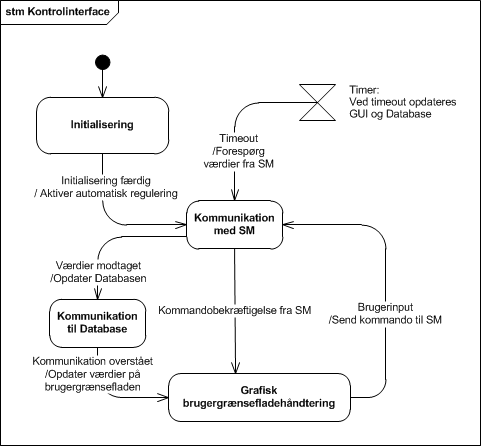
\includegraphics[width=0.6\textwidth]{billeder/KI/stm_ki}
\caption{Den simplificerede state machine for Kontrolinterfacet fra Systemarkitekturen}
\label{fig:KI-stm}
\end{figure}

State machinen er god til at få en forståelse for programmet, men for at komme videre må den uddybes væsentligt. Det første trin i designfasen har derfor været at udarbejde en mere detaljeret state machine. Resultatet kan ses i Kontrolinterface-afsnittet i dokumentationsdokumentet for Detaljeret Software Design.

Det videre skridt er at udarbejde et klassediagram for programmet. Klassediagrammet er ligesom state machines først lavet i en simplificeret version og dernæst i en detaljeret. Det første kan ses på figur \ref{fig:kd_simpel} med en beskrivelse af hver klasse i tabel \ref{tabel:ki-klasser}.\\

\begin{figure}[htbp]
\centering
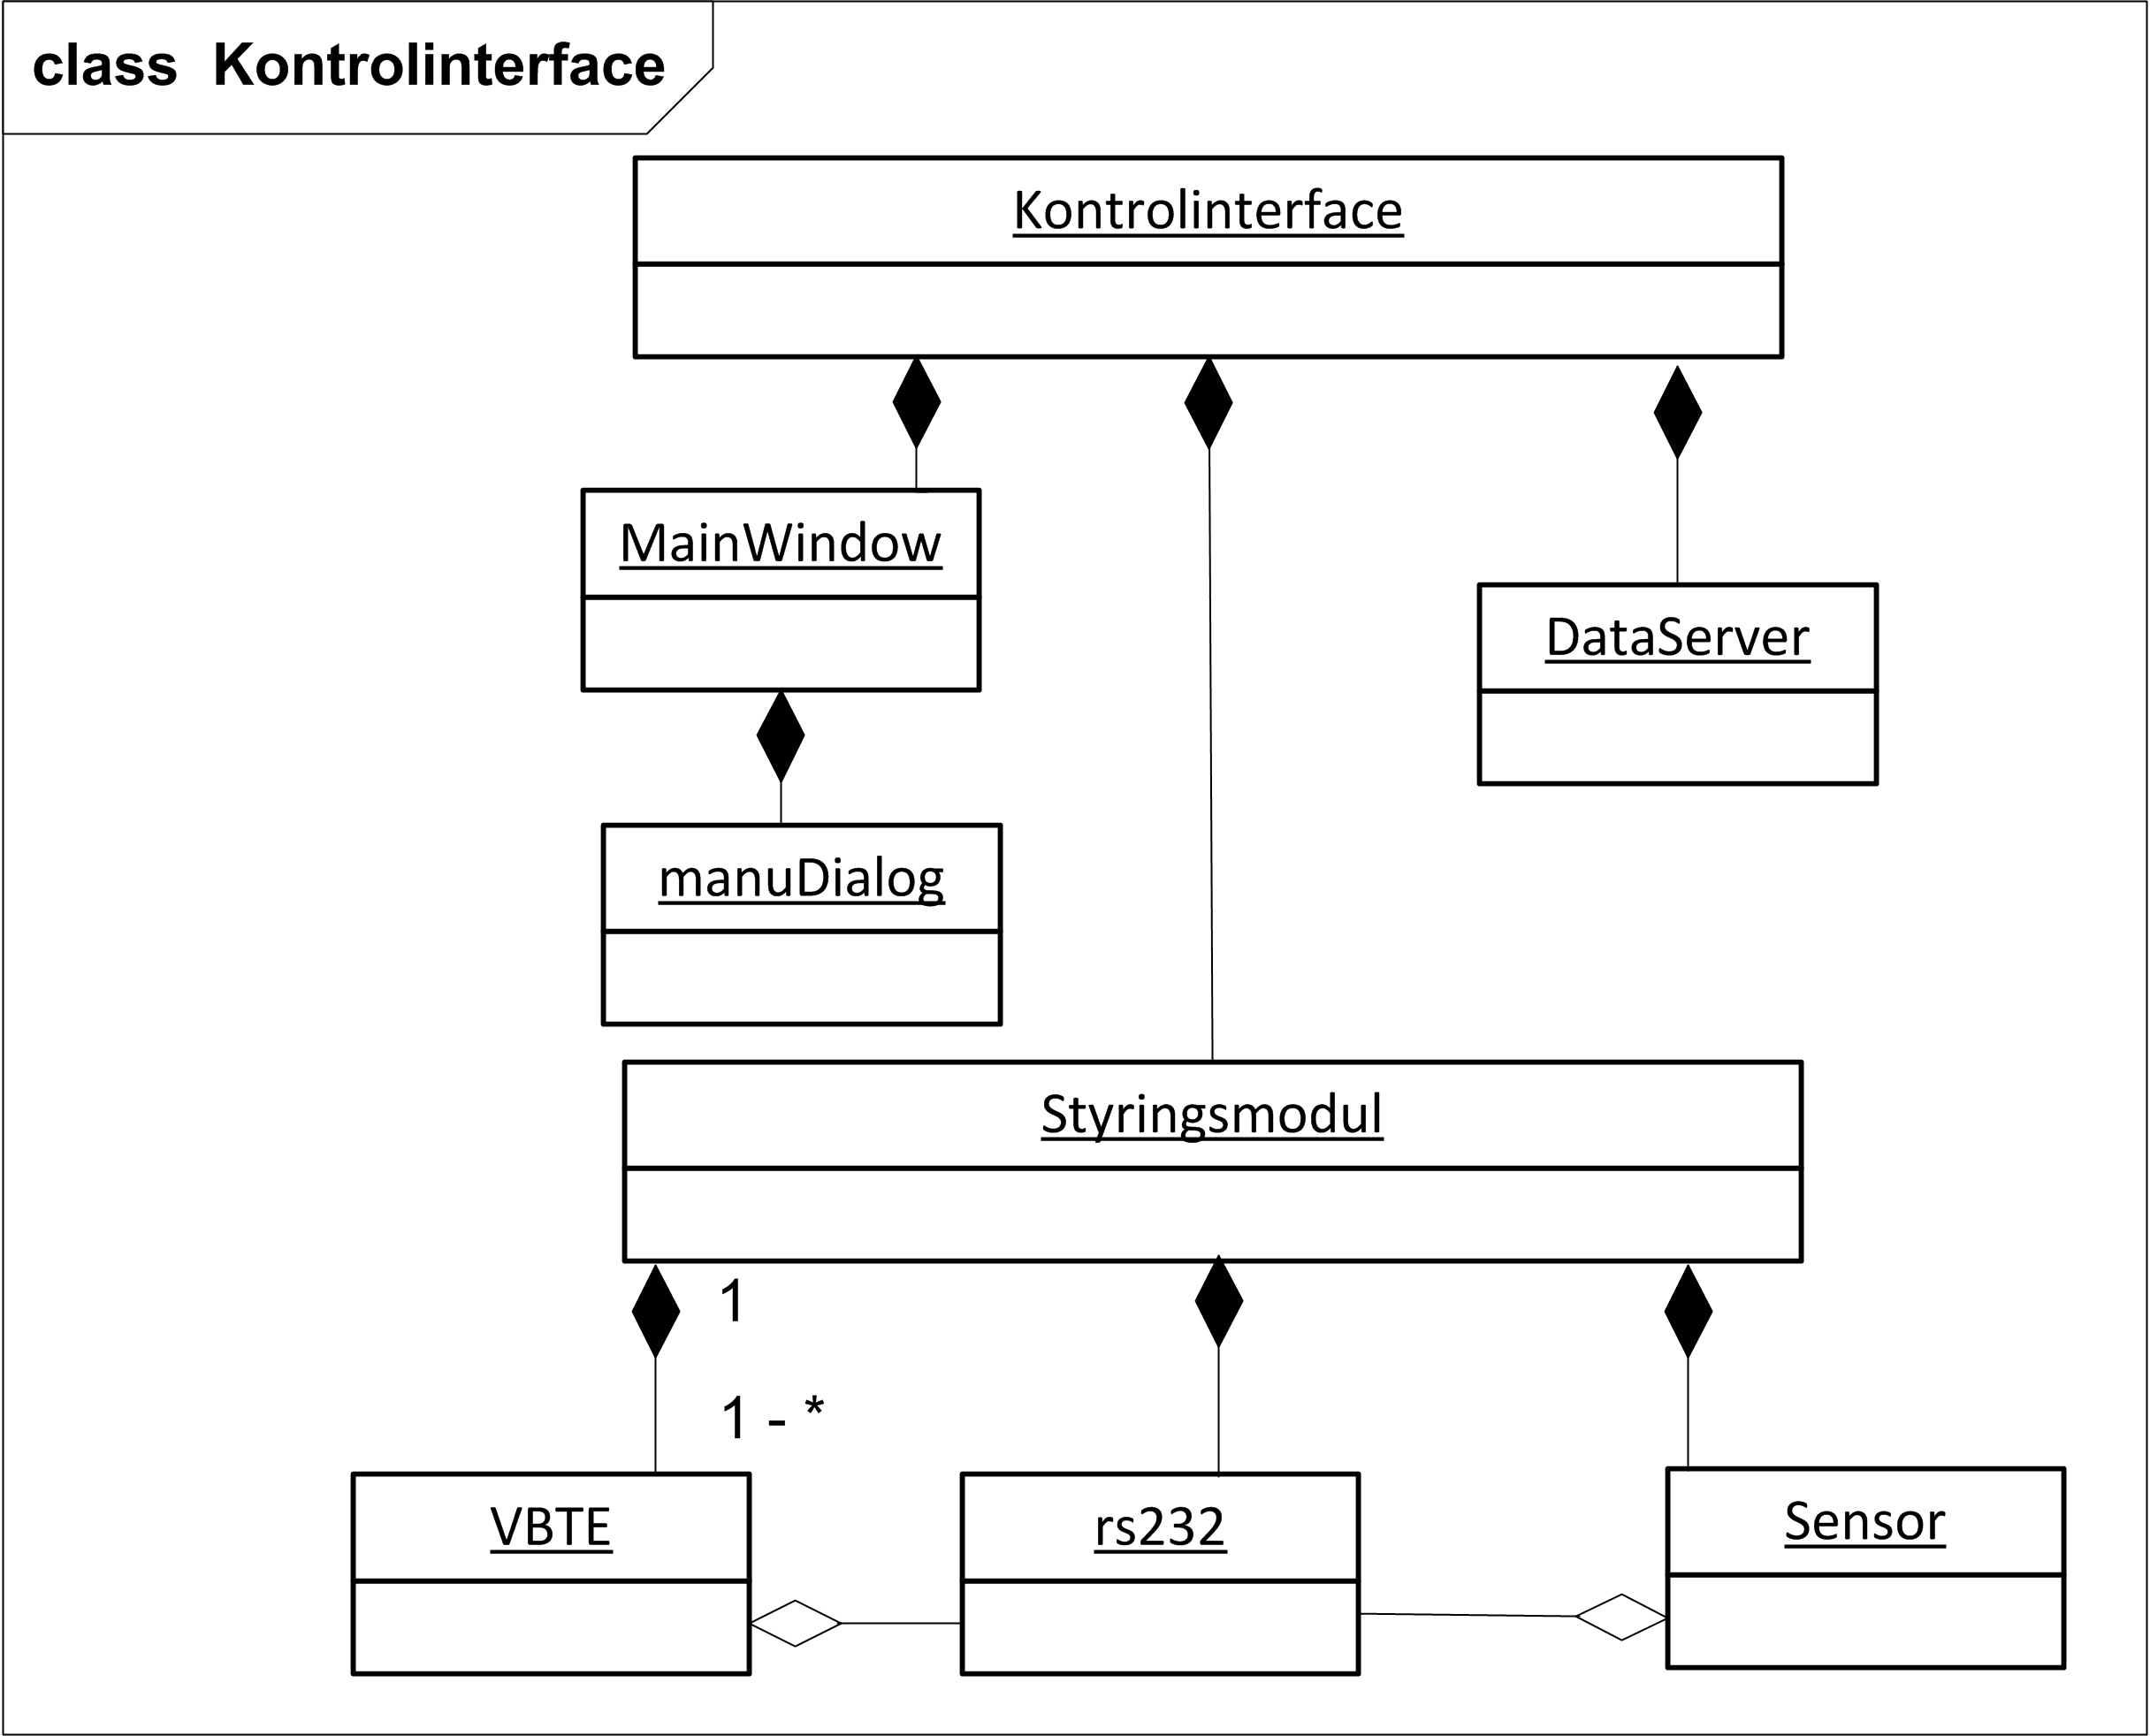
\includegraphics[width=0.5\textwidth]{billeder/KI/klassediagram_simpel}
\caption{Det simple klassediagram for Kontrolinterfacet. Beskrivelse af hver klasse i tabel \ref{tabel:ki-klasser}}
\label{fig:kd_simpel}
\end{figure}
 
\begin{table}[htbp]
\centering
\rowcolors{1}{white}{light-gray}
\begin{tabular}{| p{3cm}  p{12cm}|}
\multicolumn{2}{l}{{\Large Kontrolinterfacets klasser}} \\\hline
Kontrolinterface:&Programmets hovedklasse. Eksisterer for at rydde op i main-funktionen.\\\hline
DataServer:&Står for alt TCP-kommunikationen med databasen. Oprettes af KI-klassen\\\hline
Styringsmodul:&Oprettes af KI og opretter VBTE-, Sensor- og RS232klasserne.\\\hline
Sensor:&Oprettes af SM og er ansvarlig for hældningsværdien.\\\hline
VBTE:&Der eksisterer et VBTE-objekt for hvert fysisk VBTE-modul. Det er objektets ansvar at holde styr på værdierne for sit VBTE-modul.\\\hline
RS232:&Objektet oprettes af SM-klassen og VBTE- og Sensorobjekterne har en delt association til den. Objektet har ansvaret for kommunikationen med det fysiske SM-modul. Objektet formidler sig på en protokol forstået den kommunikationsansvarlige kode på SM-modulet. Protokollen kan ses i dokumentet for det detaljerede softwaredesign.\\\hline
MainWindow:&Oprettes af KI-klassen. Kontrollerer og overvåger den grafiske brugergrænsefalde.\\\hline
manudialog:&Oprettes af MainWindow og styrer den dialog, der fremkommer når man ønsker en manuel hældningsregulering.\\\hline
\end{tabular}
\caption{Kontrolinterfacets klasser}
\label{tabel:ki-klasser}
\end{table}

Klassediagrammet på figur \ref{fig:kd_simpel} afspejler et program designet med forbillede i det samlede system. Dette er gjort for at trække på de løsninger der er fundet i forbindelse med det fulde system. \\
Det ses hvordan hovedklassen er Kontrolinterfacet. Alt andet oprettes enten direkte af Kontrolinterface-klassen eller af en klasse oprettet af samme. Kontrolinterfacet har kun kontakt til brugergrænsefladen (MainWindow), Styringsmodulet og DataServer. Kommunikationen mellem Kontrolinterface-klassen og Styringsmodul spejler den kommunikation der er imellem de fysiske blokke Kontrolinterface og Styringsmodul i det samlede system.\\

Det gælder for VBTE-, SM- og Sensor-klasserne at når der efterspørges en af de værdier, klassen har ansvaret for, så benyttes RS232-objektet til at fremskaffe disse værdier ved hjælp af den serielle kommunikationsprotokol. 


\subsubsection{Grafisk brugergrænseflade}
I denne sektion vil der kort blive gennemgået det vigtigste vindue i den grafiske brugergrænseflade; hovedvinduet. En gennemgang af de resterende vinduer vil kunne findes i Softwaredesign Appendix A: Kontrolinterface.
På figur \ref{fig:hovedvindue} er hovedvinduet vist. Her er vinduets elementer indrammet. Herefter vil hovedvinduets elementer blive beskrevet.

\begin{figure}[H]
\centering
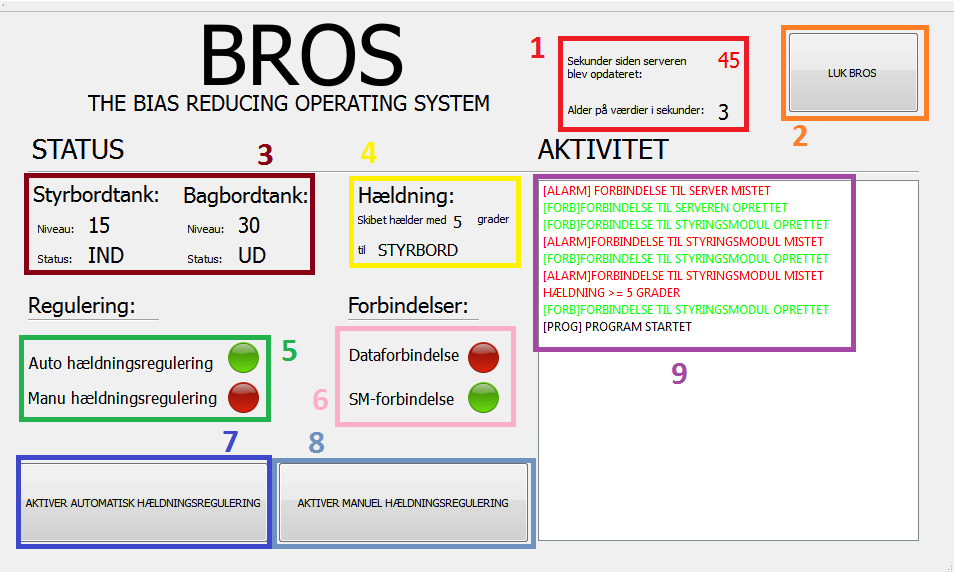
\includegraphics[width=0.7\textwidth]{billeder/KI/hovedvindue}
\caption{På figuren ses hovedvinduet for Kontrolinterface-programmet}
\label{fig:hovedvindue}
\end{figure}

\textcolor{red}{\textbf{1: Forsinkelse i sekunder}}\\
Det øverste tal fortæller tiden i sekunder siden serveren sidst er blevet opdateret succesfuldt.
Nedenunder udskrives tiden i sekunder siden værdierne i boks tre og fire er blevet opdateret.

\textcolor{Orange}{\textbf{2: Nedlukningsknap}}\\
Anvendes til at lukke programmet. Programmet åbner dialogen som kan ses i Designdokumentet, Appendix A.

\textcolor{brown}{\textbf{3: Vandballasttankene}}\\
Her kan status for vandballasttankene aflæses. Niveauet er hvor fyldt tanken er angivet i procent. Hvis niveauet er over 70\% skrives tallet med rødt.
Status angiver vandets flow i tanken: IND/UD/LUKKET.

\textcolor{yellow}{\textbf{4: Hældningssensor}}\\
Værdien for hældningen af skibet angives i antal grader og i hvilken side skibet hælder.

\textcolor{green}{\textbf{5: Reguleringsstatus}}\\
Her angives hvorvidt automatisk eller manuel hældningsregulering er aktiveret. Der vil altid kun være en og kun en af disse aktiveret. Derfor vil der altid være en rød og en grøn indikator tændt. I dette eksempel er den automatisk hældningsregulering aktiveret.
	
\textcolor{pink}{\textbf{6: Forbindelser}}\\
Indikerer hvorvidt der er forbindelse til Styringsmodulet og serveren. Dataforbindelse er rød hvis det ikke lykkedes at oprette forbindelse til serveren ved sidste forsøg.
SM-forbindelse er rød hvis det ikke lykkedes at få de ventede svar fra Styringsmodulet.
I denne situation er der forbindelse til styringsmodulet, men ikke serveren.

\textcolor{blue}{\textbf{7: Automatisk reguleringsknap}}\\
Ved tryk på denne knap vil man komme til en dialog hvor man beder bekræfte at man ønsker at gå væk fra manuel hældningsregulering. Hvis automatisk regulering allerede er aktiveret vil man få dette af vide i en dialog. Dialogerne kan ses i Designdokumentet, Appendix A.

\textcolor{BlueGreen}{\textbf{8: Manuel reguleringsknap}}\\
Bringer dig til en dialog hvori hældningen vælges fra 0.5 grader til 2.5 grader. Herefter vælges siden skibet skal hælde til. Dialogen kan ses i Designdokumentet, Appendix A.

\textcolor{purple}{\textbf{9: Aktivitetslog}}\\
Her udskrives vigtige hændelser i programmet med farvekoder. I dette eksempel kan det ses hvordan alarmer skrives med rødt og oprettede forbindelser skrives med grønt.

%%%%%%%%%%%%%%%%%%%%%%%%%%%%
%%%%%%%%%% VBTE %%%%%%%%%%%%
%%%%%%%%%%%%%%%%%%%%%%%%%%%%
\subsection{VBTE}
I dette afsnit beskrives design og implementering af VBTE for både software og hardware. 
\subsubsection{Hardware}
Til VBTE'en er der blevet designet hardware til at styre de to ventiler samt den keramiske ultralydstransmitter og receiver. Hardware er blevet udfærdiget i to dele. Den ene er programmeret hardware på PSoC'en, den anden er hardware uden for PSoC'en. Hardware designprocessen til VBTE'en gik igennem 3 faser:
\begin{enumerate}
\item Overordnet design
\item Nedbrydning af blokke
\item Opbygning af design
\end{enumerate}
Gennem disse faser er designet blevet udfærdiget. Fremgangsmåden er anvendt for at overskueligtgøre systemet og lette arbejdet ved at dele systemet op i små dele. På \textit{figur \ref{fig:HWVBTE}} ses det overordnede design af VBTE'en. Der vil i rapporten tages udgangspunkt i ventilkredsen samt receiverdriveren på PSoC'en.
\begin{figure}[H]
\centering
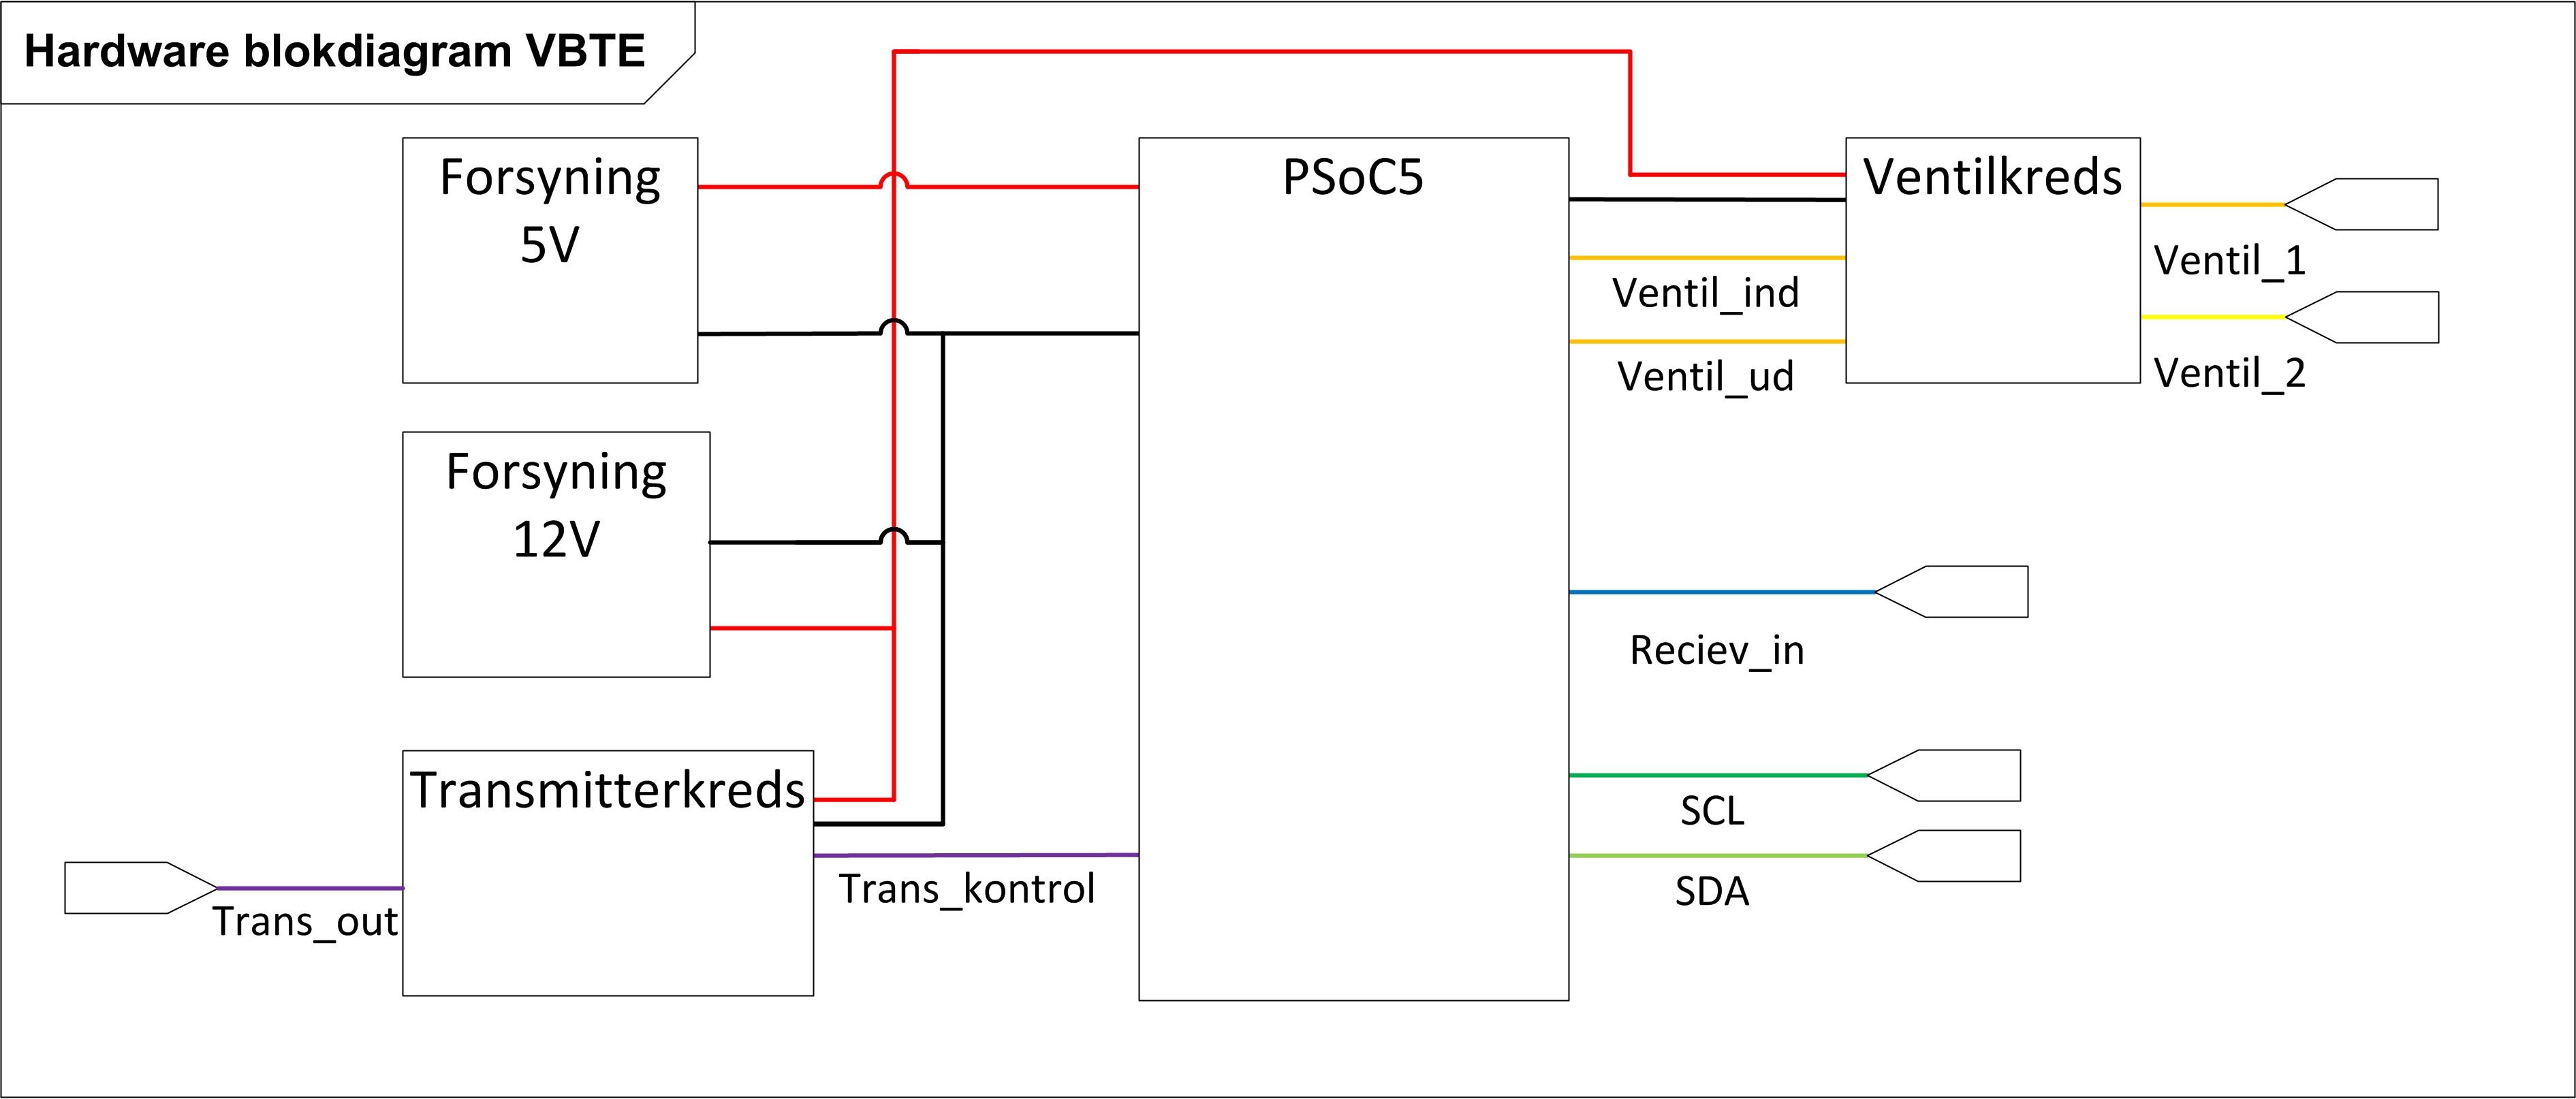
\includegraphics[width = 0.9\textwidth]{billeder/HWVBTE}
\caption{Illustrering af overordnet design af hardware på VBTE.}
\label{fig:HWVBTE}
\end{figure}
\subsubsection{Hardware på PSoC'en}
Hardware opbygget på PSoC'en kunne uden problemer være blevet designet uden for PSoC'en, men PSoC miljøet gør det meget nemt at arbejde med mange forskellige elementer. Der vil i rapporten ligges vægt på transmitterkredsen samt receiverkredsen. På figur \ref{fig:PSOCHW} ses hardware designet på PSoC'en.
\begin{figure}[H]
\centering
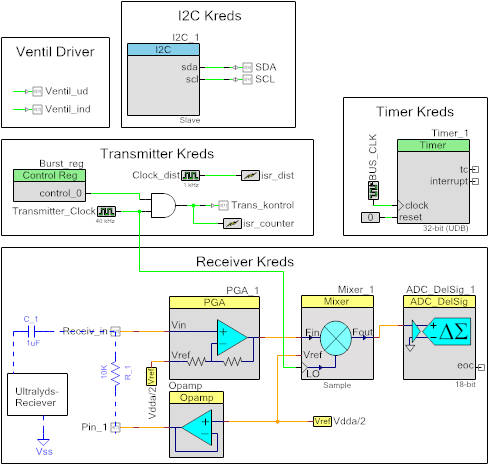
\includegraphics[width=0.7\textwidth]{billeder/PSOC_Hardware}
\caption{Hardware på PSoC'en.}
\label{fig:PSOCHW}
\end{figure}
\subsubsection{Transmitterkreds}
Transmitterkredsen står for at sende burst samt at time hvert burst.  Dette opnåes med to clocks, en AND gate, en output pin samt et kontrol register. Transmitterclocken er indstillet til 40kHz da ultralydstransmitteren, ifølge databladet, opererede ved $\SI{40}{kHz}\pm\SI{1}{kHz}$. Clocken er blevet målt på oscilloskop til $\SI{40.3}{kHz}$. Burst kontrolregisteret er anvendt til at AND'e clocken ud på trans\_kontrol pinden.\\
Clock\_dist interruptrutinen sørger for at tælle en variabel op der anvendes i main til at kalde burst funktionen. Dette gøres for at lave et nonblocking delay så andet kan køres på PSoC'en mens et burst er sendt afsted og der afventes detektion.
\subsubsection{Receiverkreds}
Receiverkredsen modtager signalet fra ultralydsreceiveren og omsætter det til en detektion. Dette sker efter følgende opskrift:\\
Løfte signalet $\rightarrow$ Forstærkning $\rightarrow$ Mixning.\\
Signalet bliver løftet på til $\frac{Vdda}{2}$ fordi PSoC'en ikke kan arbejde med værdier under Vssa (GND). Dette gøres ved hjælp af en kondensator, en modstand og en spændingsfølger med $\frac{Vdda}{2}$ på det positive ben.\\
Efter signalet er løftet, bliver det forstærket op af en PGA. Den første forstærkning, fundet i teknologiundersøgelsen, viste sig at være for lav og forstærkningen blev justeret til 32. Problemet heri ligger at et meget klart signal vil kunne få systemet til at gå i mætning. Men dette ser ikke ud til at ske.\\
Herefter bliver signalet mixet med $\SI{40}{kHz}$ og filtreret. Efter mixeren giver det, stort set, en DC og summen af de to signaler. Filteret er indbygget i Delta-Sigma ADC'en og har en knækfrekvens ved $\frac{Sample frekvens}{3}$. For at være sikker på at det meste af signalet er kommet over regnes der en opladningstid på filteret til $\SI{1/4}{ms}$. Efter undersøgelser af signalet ind på ADC'en blev en spænding på $\SI{0.3}{V}$ valgt til at representere en detektion.

\subsubsection{Hardware uden for PSoC'en}
Uden for PSoC'en er der lavet 2 hardwareblokke (Ventilkreds og transmitterkreds). Disse har til ansvar at omsætte et kontrolsignal til en større spænding over de respektive enheder. Herunder vil der blive fokuseret på ventilkredsen.
\begin{figure}[H]
	\centering
	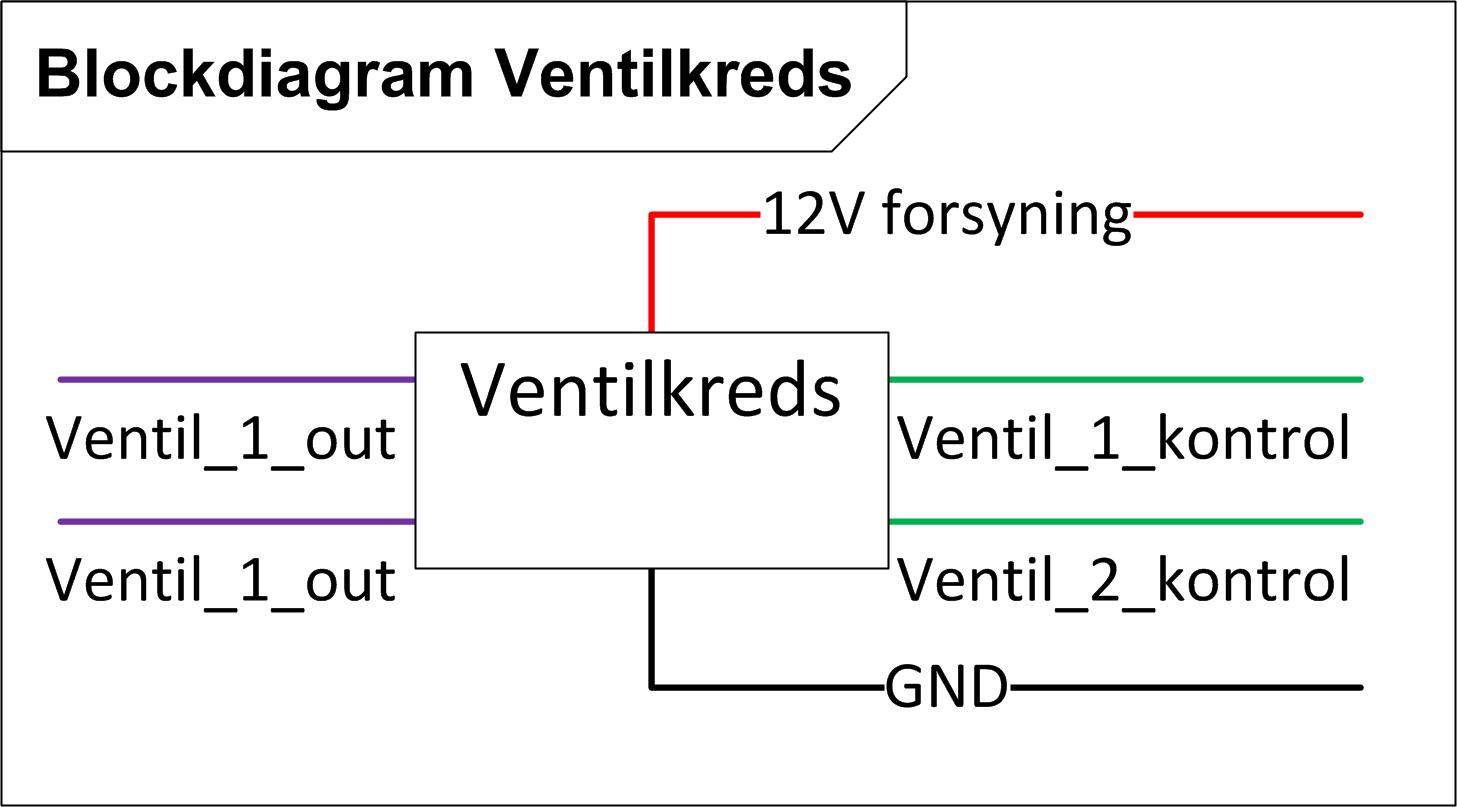
\includegraphics[width=0.40\textwidth]{billeder/Ventilblok}
	\caption{Hardwareblok for ventil}
	\label{fig:Ventilblok1}
\end{figure}
\subsubsection{Ventilkreds}
Ventilkredsen får to kontrolsignaler fra PSoC'en og disse skal styre de to ventiler. Ventilerne monteret på kredsen er fra Danfoss og er af modellerne EV210A-1.2 og EV210A-4.5. Disse ventiler drives ved 12V 0.4A. Der er valgt en BD139 transistor til at forstærke signalet op. Denne har en forstærkning mellem 40 og 160 (aflæst fra databladet\footnote{Se bilag/BD139.pdf}). IO's på PSoC'en kan maksimalt trække en strøm på $\SI{4}{mA}$ og det vil i værste tilfælde ikke være nok til at trække ventilerne.\\
Der er derfor lavet en darlington kobling for at mindske belastningen af PSoC'en og for at sikre at der bliver lukket nok op for transistoren. Dette er gjort med en transistor af typen BC547. Transistorne er valgt ud fra pris og tilgængelighed. Der var først valgt en MOSFET IRLZ44n men denne var både for dyr og kunne klare en unødvendig stor effekt. Det smarte ved MOSFET'en er dog at den er spændingsstyret i forhold til de to andre transistorer. 

%\subsubsection{Transmitterkreds}
%Transmitterkredsen anvender ultralydstranduceren som en højtaler. Denne er koblet over transistoren (Her anvendes også en BD139).\\
%Via. kontrolsignalet fra PSoC'en, der bliver sendt ud ved $\SI{40}{kHz}$, bliver der sat en spænding over transduceren.\\ 
%Forsyningen hertil trækkes fra samme forsyning som ventilkredsen der bliver leveret fra powersuply'en. Ud fra databladet er der aflæst en ohmsk modstand på omtrendt $\SI{10}{k}\Omega$. Derfor kan PSoC'en uden problemer selv trække denne kreds.
%\begin{figure}[H]
%\centering
%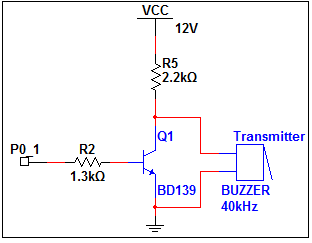
\includegraphics[width = .5\textwidth]{billeder/transmitterkreds}
%\caption{Transmitterkreds}
%\end{figure}
%For yderligere detaljer vedrørende hardware på VBTE henvises til \textit{Deltajeret hardware design}.

\subsubsection{Software}
Softwaren til VBTE modulet er blevet designet til at kunne opfylde kravene i kravspecifikationen samt arkitekturen i systemarkitekturen. Den er blevet designet til at passe til hardwaren så den kan kontrollere de enkelte elementer. I designfasen er der blevet udfærdiget et klassediagram samt en statemachine over funktionaliteten. På \textit{figur \ref{fig:VBTEklasse} } ses klassediagramet for VBTE modulets software.
\begin{figure}[H]
\centering
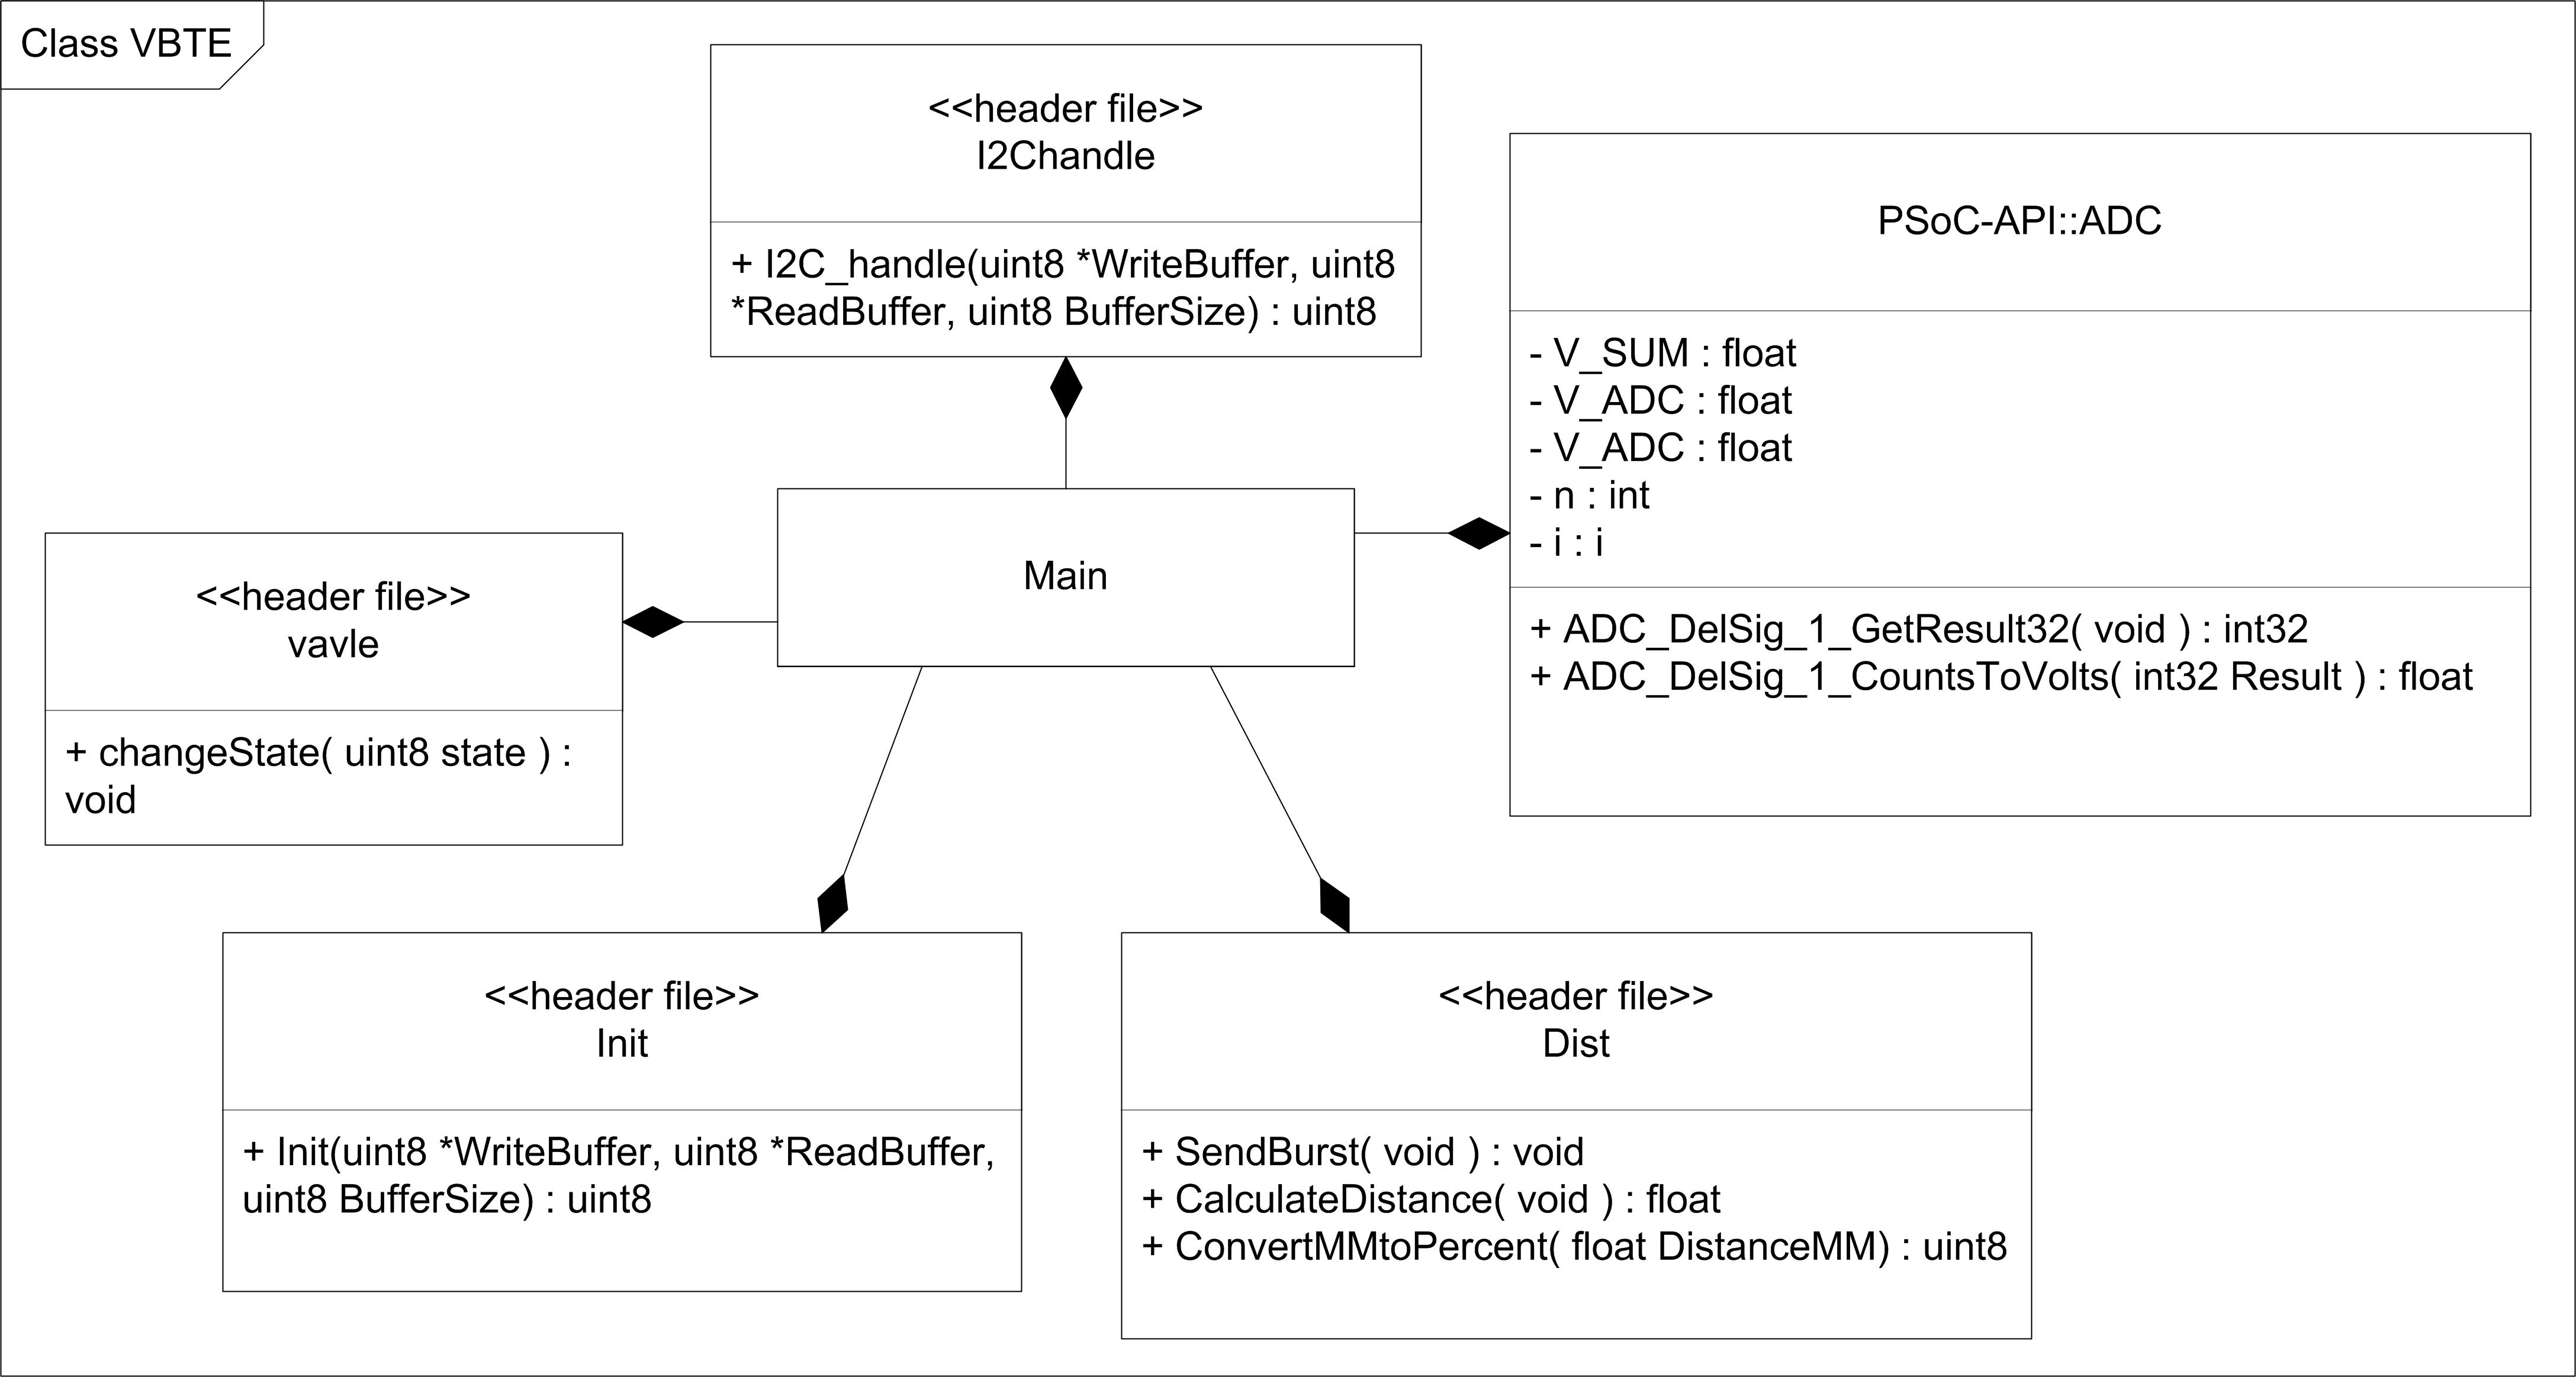
\includegraphics[width=.8\textwidth]{billeder/ClassVBTE}
\caption{Klassediagram over VBTE}
\label{fig:VBTEklasse}
\end{figure}
Selvom softwaren er skrevet i C er der lavet klasser for alle h-filer for at gøre systemet overskueligt. For detaljerede metodebeskriveler henvises til detaljeret software design.\\
For at overskueligtgøre funktionaliteten af softwaren anvendes statemachinediagrammet. Dette viser de forskellige tilstande programmet til enhver til kan befinde sig i.
\begin{figure}[H]
\centering
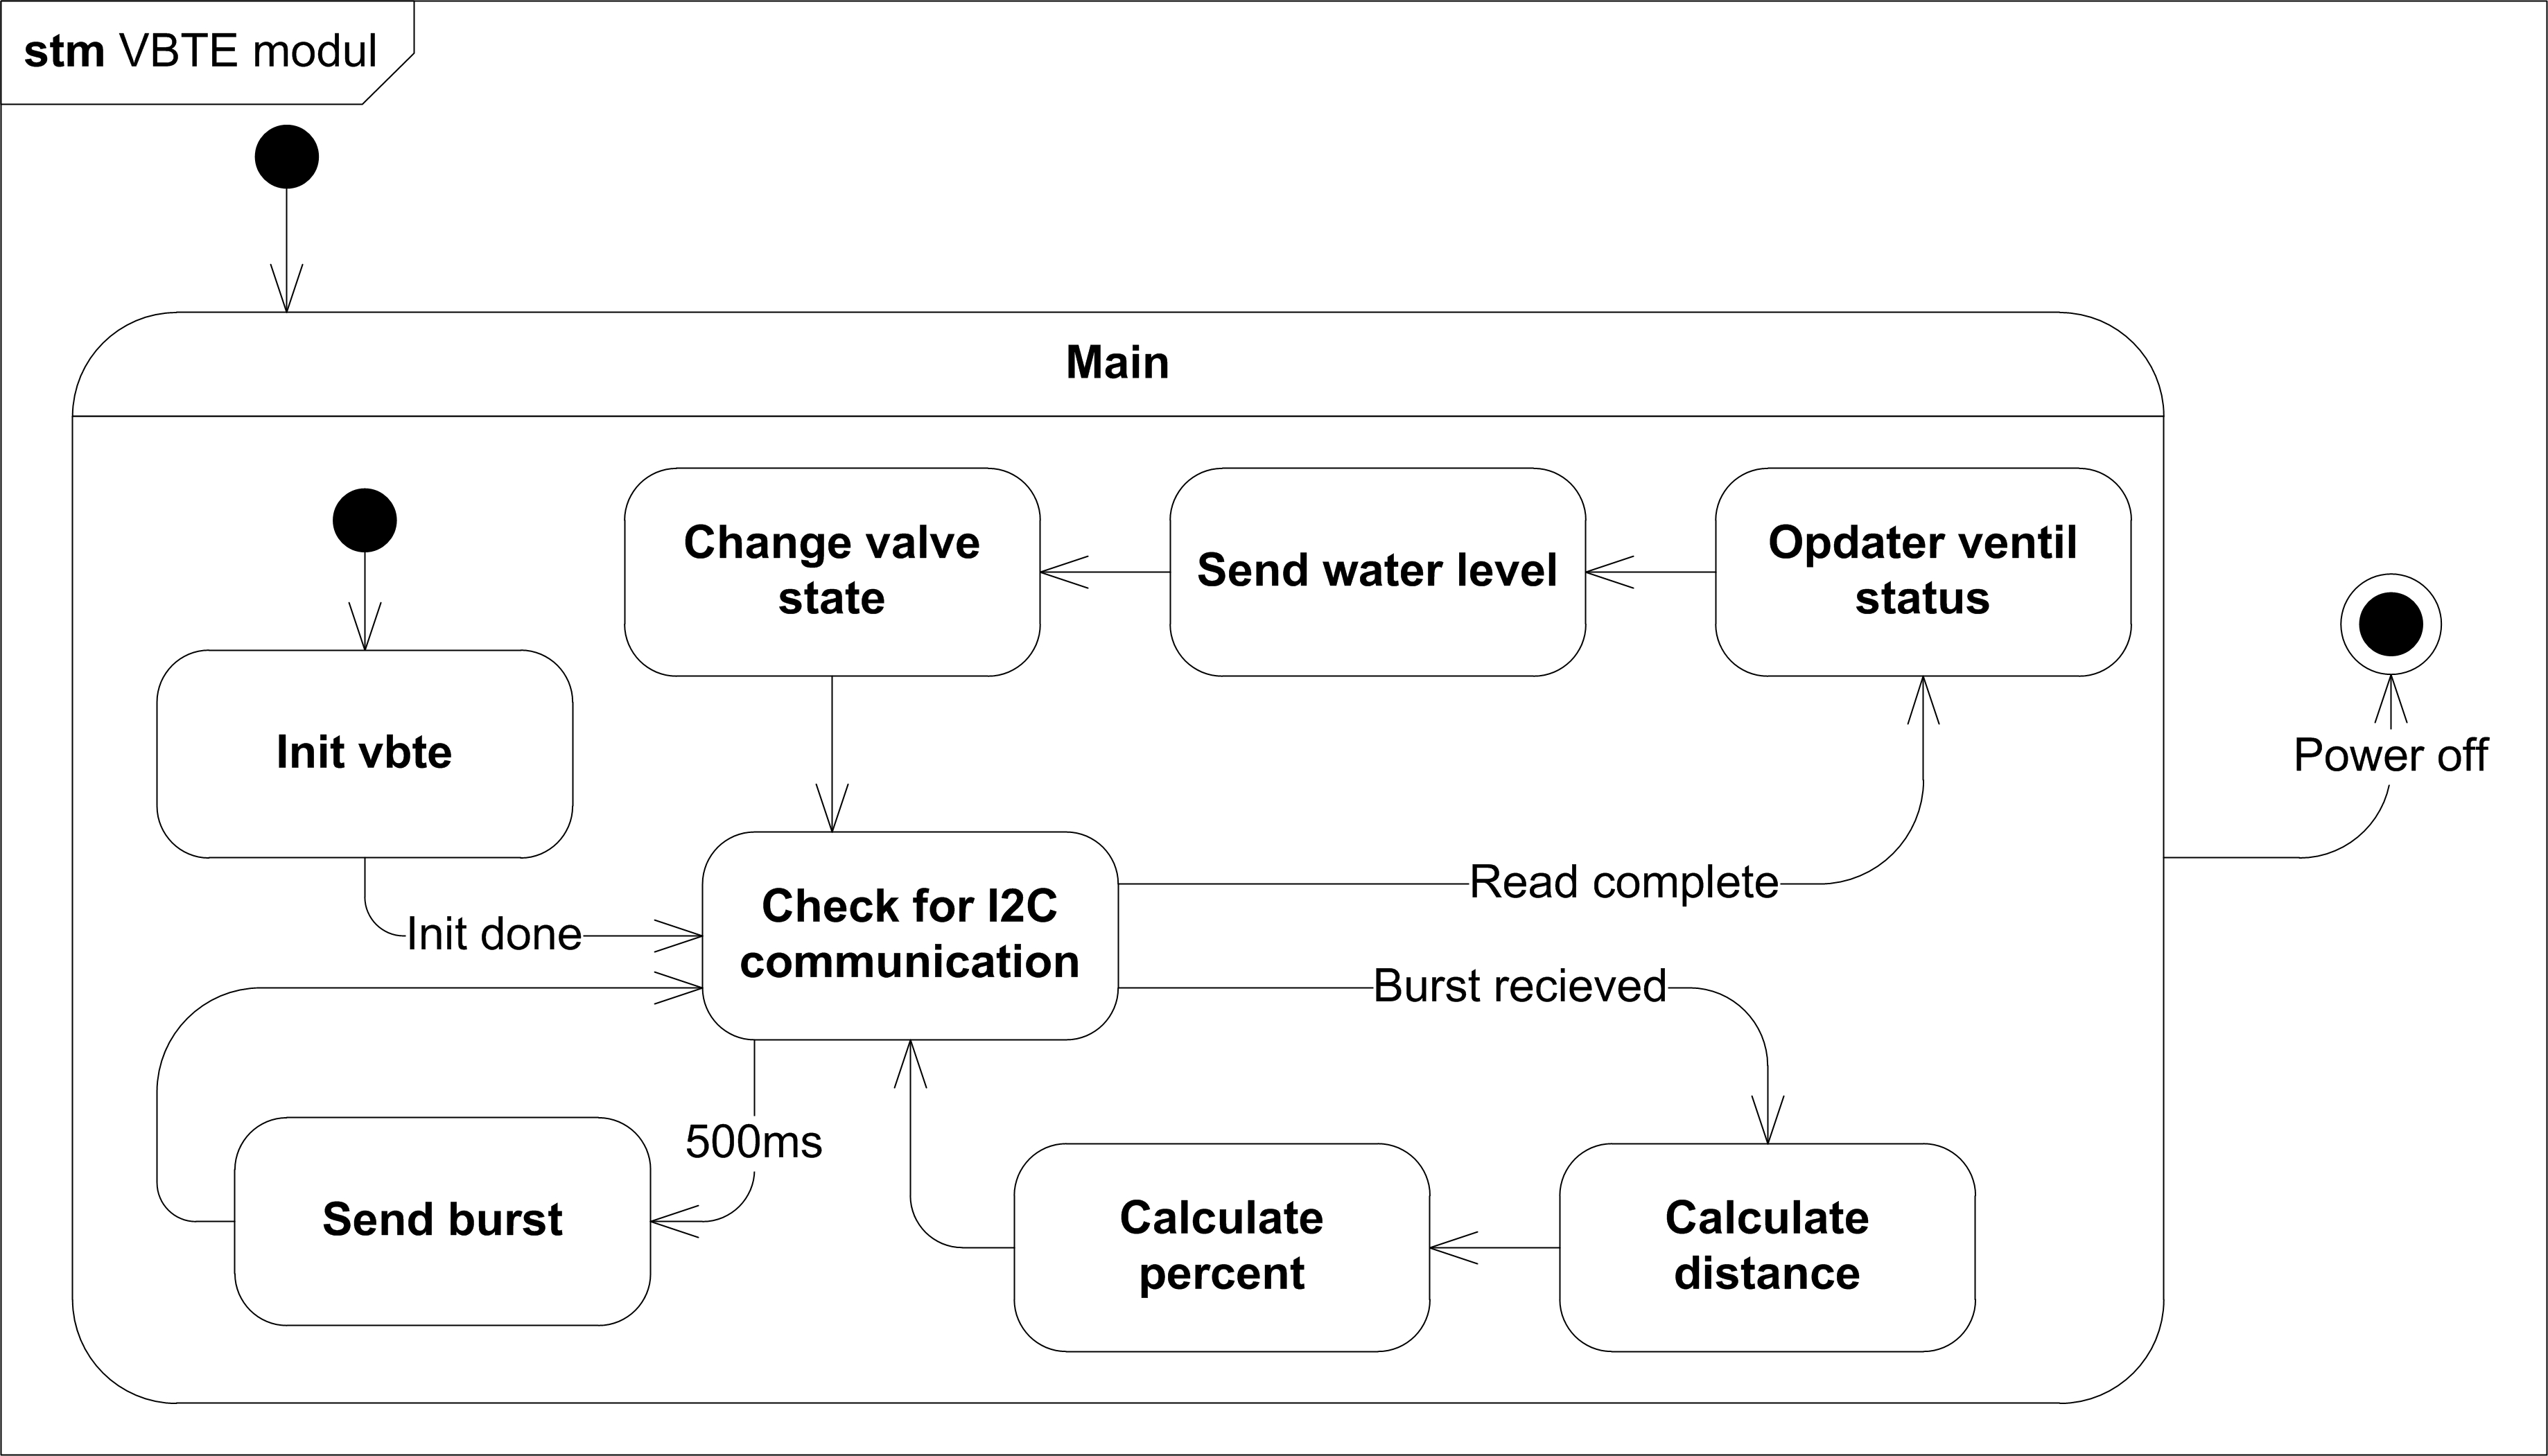
\includegraphics[width=.8\textwidth]{billeder/STMVBTE}
\caption{Statemachine for VBTE software}
\end{figure}
De forskellige betingelser der skal til for at skifte tilstand vil herefter blive beskrevet. \\
Som nævnt i hardware anvendes et interrupt til at lave et nonblocking delay på 500ms. Dette håndteres på VBTE'en i main ved hjælp af en if sætning der tjekker op på variablen fra interruptet.\\
Burst receivered bliver opnået når flaget hertil bliver sat. Dette flag bliver sat inde i ADC'ens interruptrutine når den måler en værdi der indikerer at et burst er modtaget.\\
Read complete betingelsen bliver kontrolleret inde i I2C\_handle. Heri aflæses data fra SM og omsættes til et state for ventilerne. Herefter fyldes afstanden for tankene ind i readbufferen for I2C'en med henblik på at den sendes retur. Herefter ændres ventil tilstanden så den passer med den modtagede tilstand.\\
For yderligere detaljer om software for VBTE henvises til detaljeret design dokumentation.
%%%%%%%%%%%%%%%%%%%%%%%%%%%%
%%%%%%%%%%% SM %%%%%%%%%%%%%
%%%%%%%%%%%%%%%%%%%%%%%%%%%%
\subsection{SM}
I dette afsnit beskrives design og implementering af SM modulet. SM modulet består af både software og hardware.
\subsubsection{Hardware}
SM modulets hardware består af en konverteringskreds og en PSoC. På PSoC'en er monteret et Kionix KXSC7-2050 accelerometer. Konverteringskredsen anvendes til at sende UART signaler fra PSoC til en KI modulet. Accelerometerets x-akse anvendes til hældningsmålinger for hældningssensorblokken.\\
Designfasen til SM er delt op i 3 faser:
\begin{enumerate}
\item Overordnet design
\item Nedbrydning af blokke
\item Opbygning af design
\end{enumerate}
Denne fremgangsmåde gør det muligt for en udefrakommende at følge med i processen og at kunne implementere modulet så det kan opfylde de krav der er opstillet. Ligeledes gør fremgangsmåden det lettere at overskue flere løsninger til hvert problem. på \textit{Figur~\ref{fig:SMHW1}} ses det Overordnede design og på \textit{Figur~\ref{fig:SMPSOC1}} ses PSoC blokken i SM. Der bliver efterfølgende taget udgangspunkt i Hældningssensoren. \\
\begin{figure}[H]
	\centering
	\begin{minipage}[b]{0.48\textwidth}\centering
	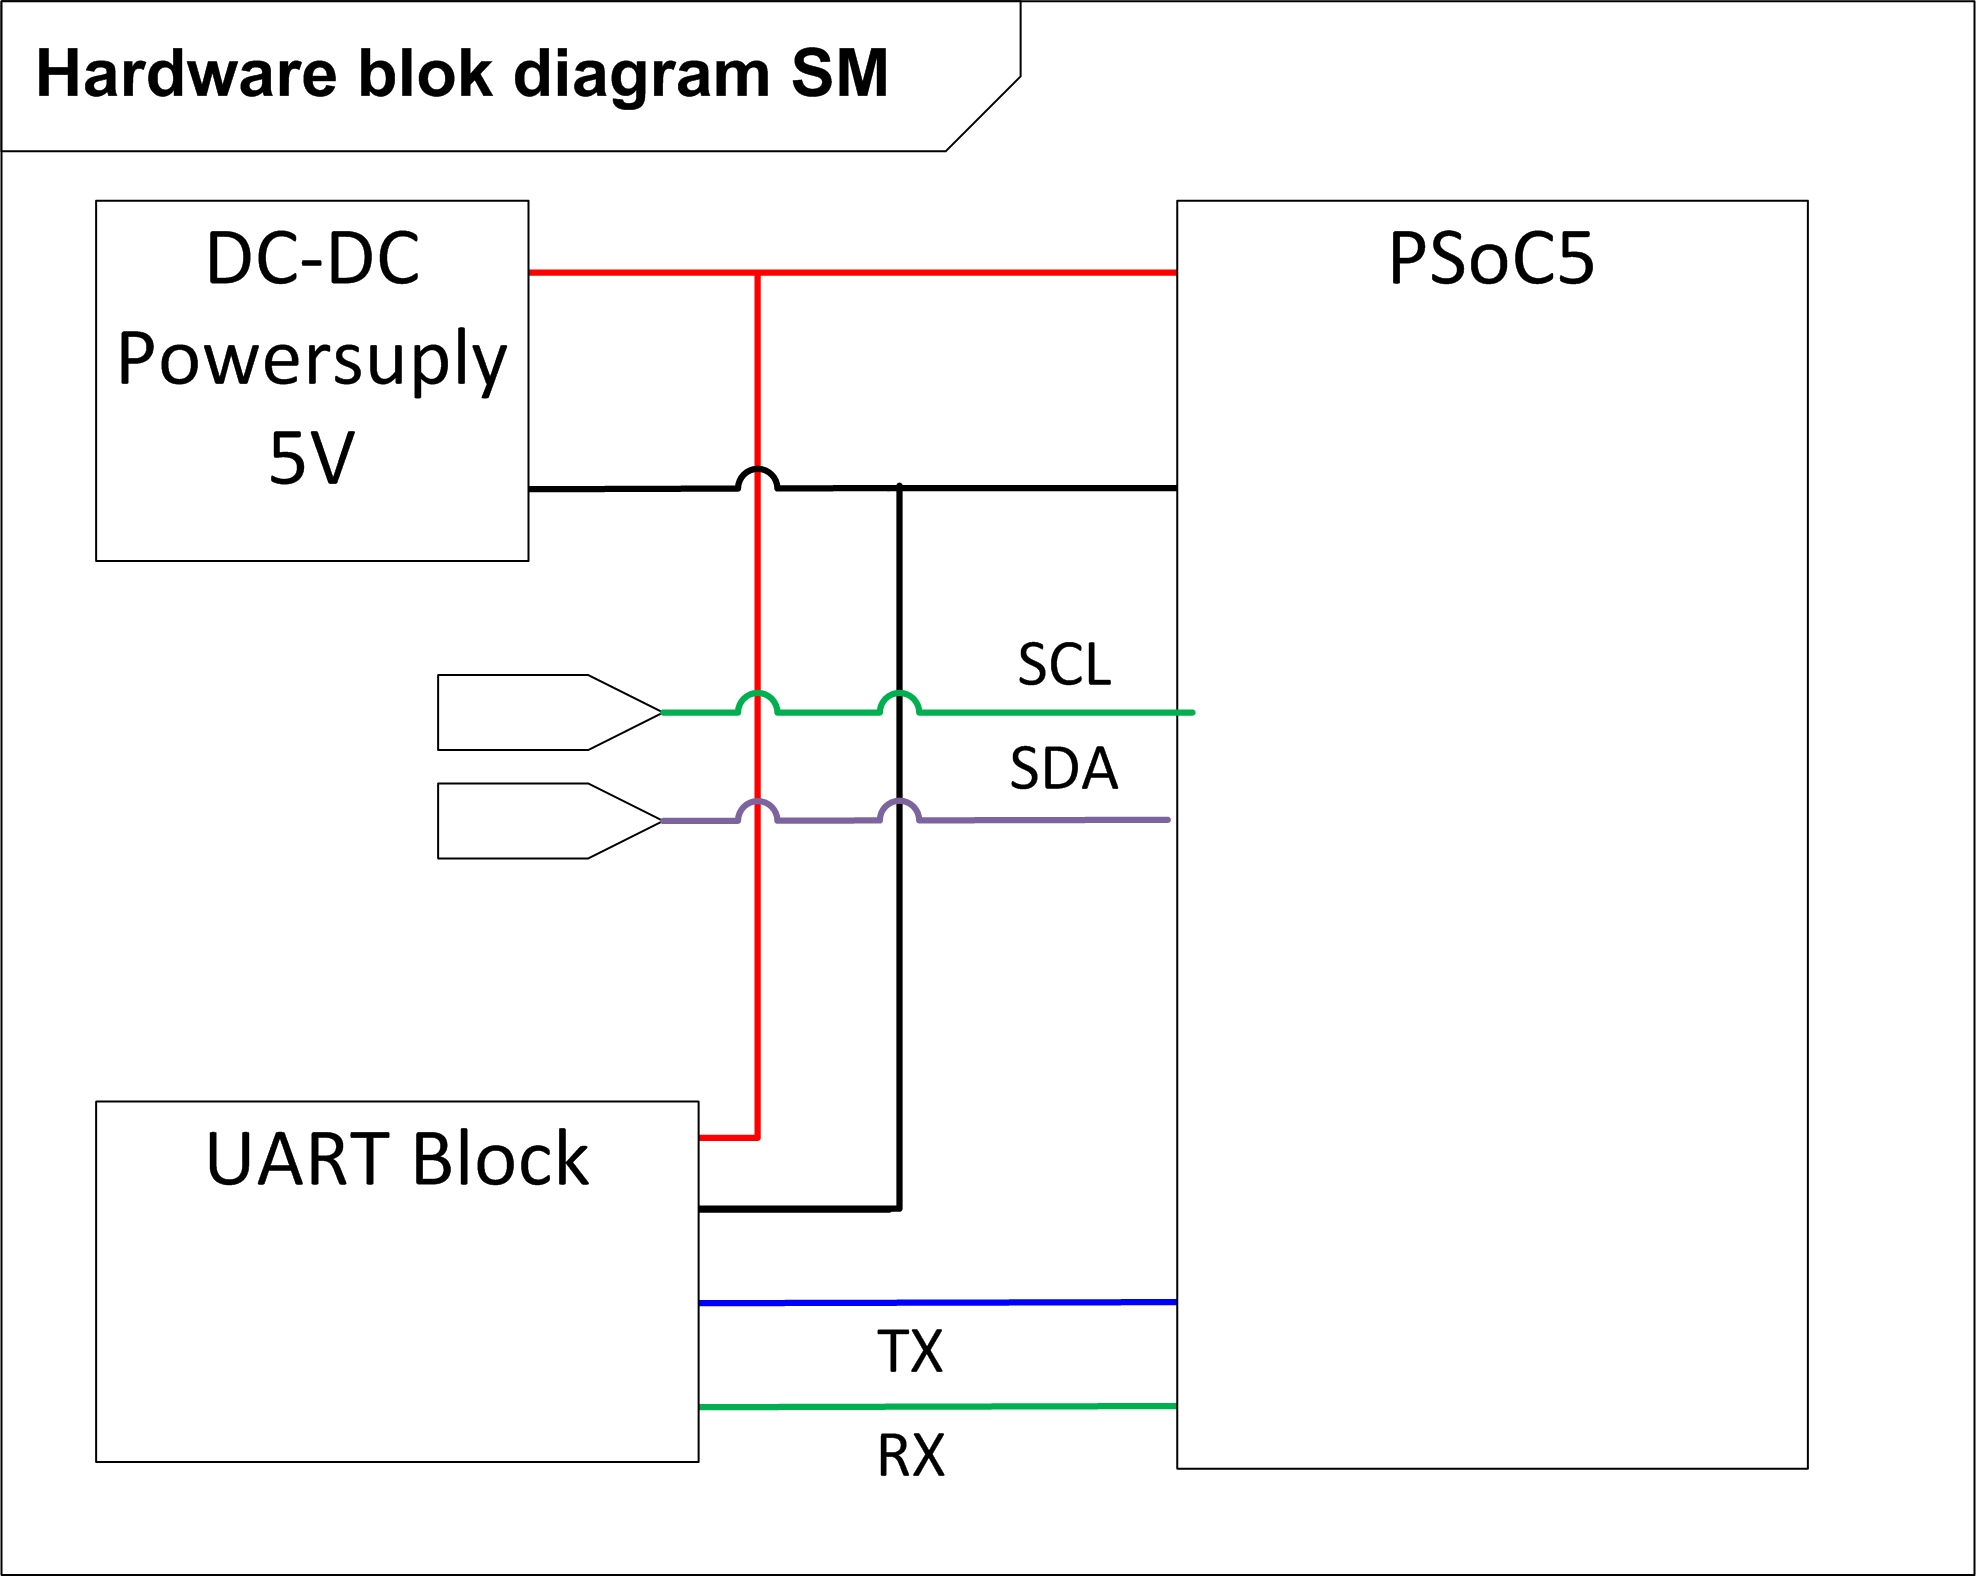
\includegraphics[width=0.80\textwidth]{billeder/SMHardware}
	\end{minipage}
	\begin{minipage}[b]{0.48\textwidth}\centering
	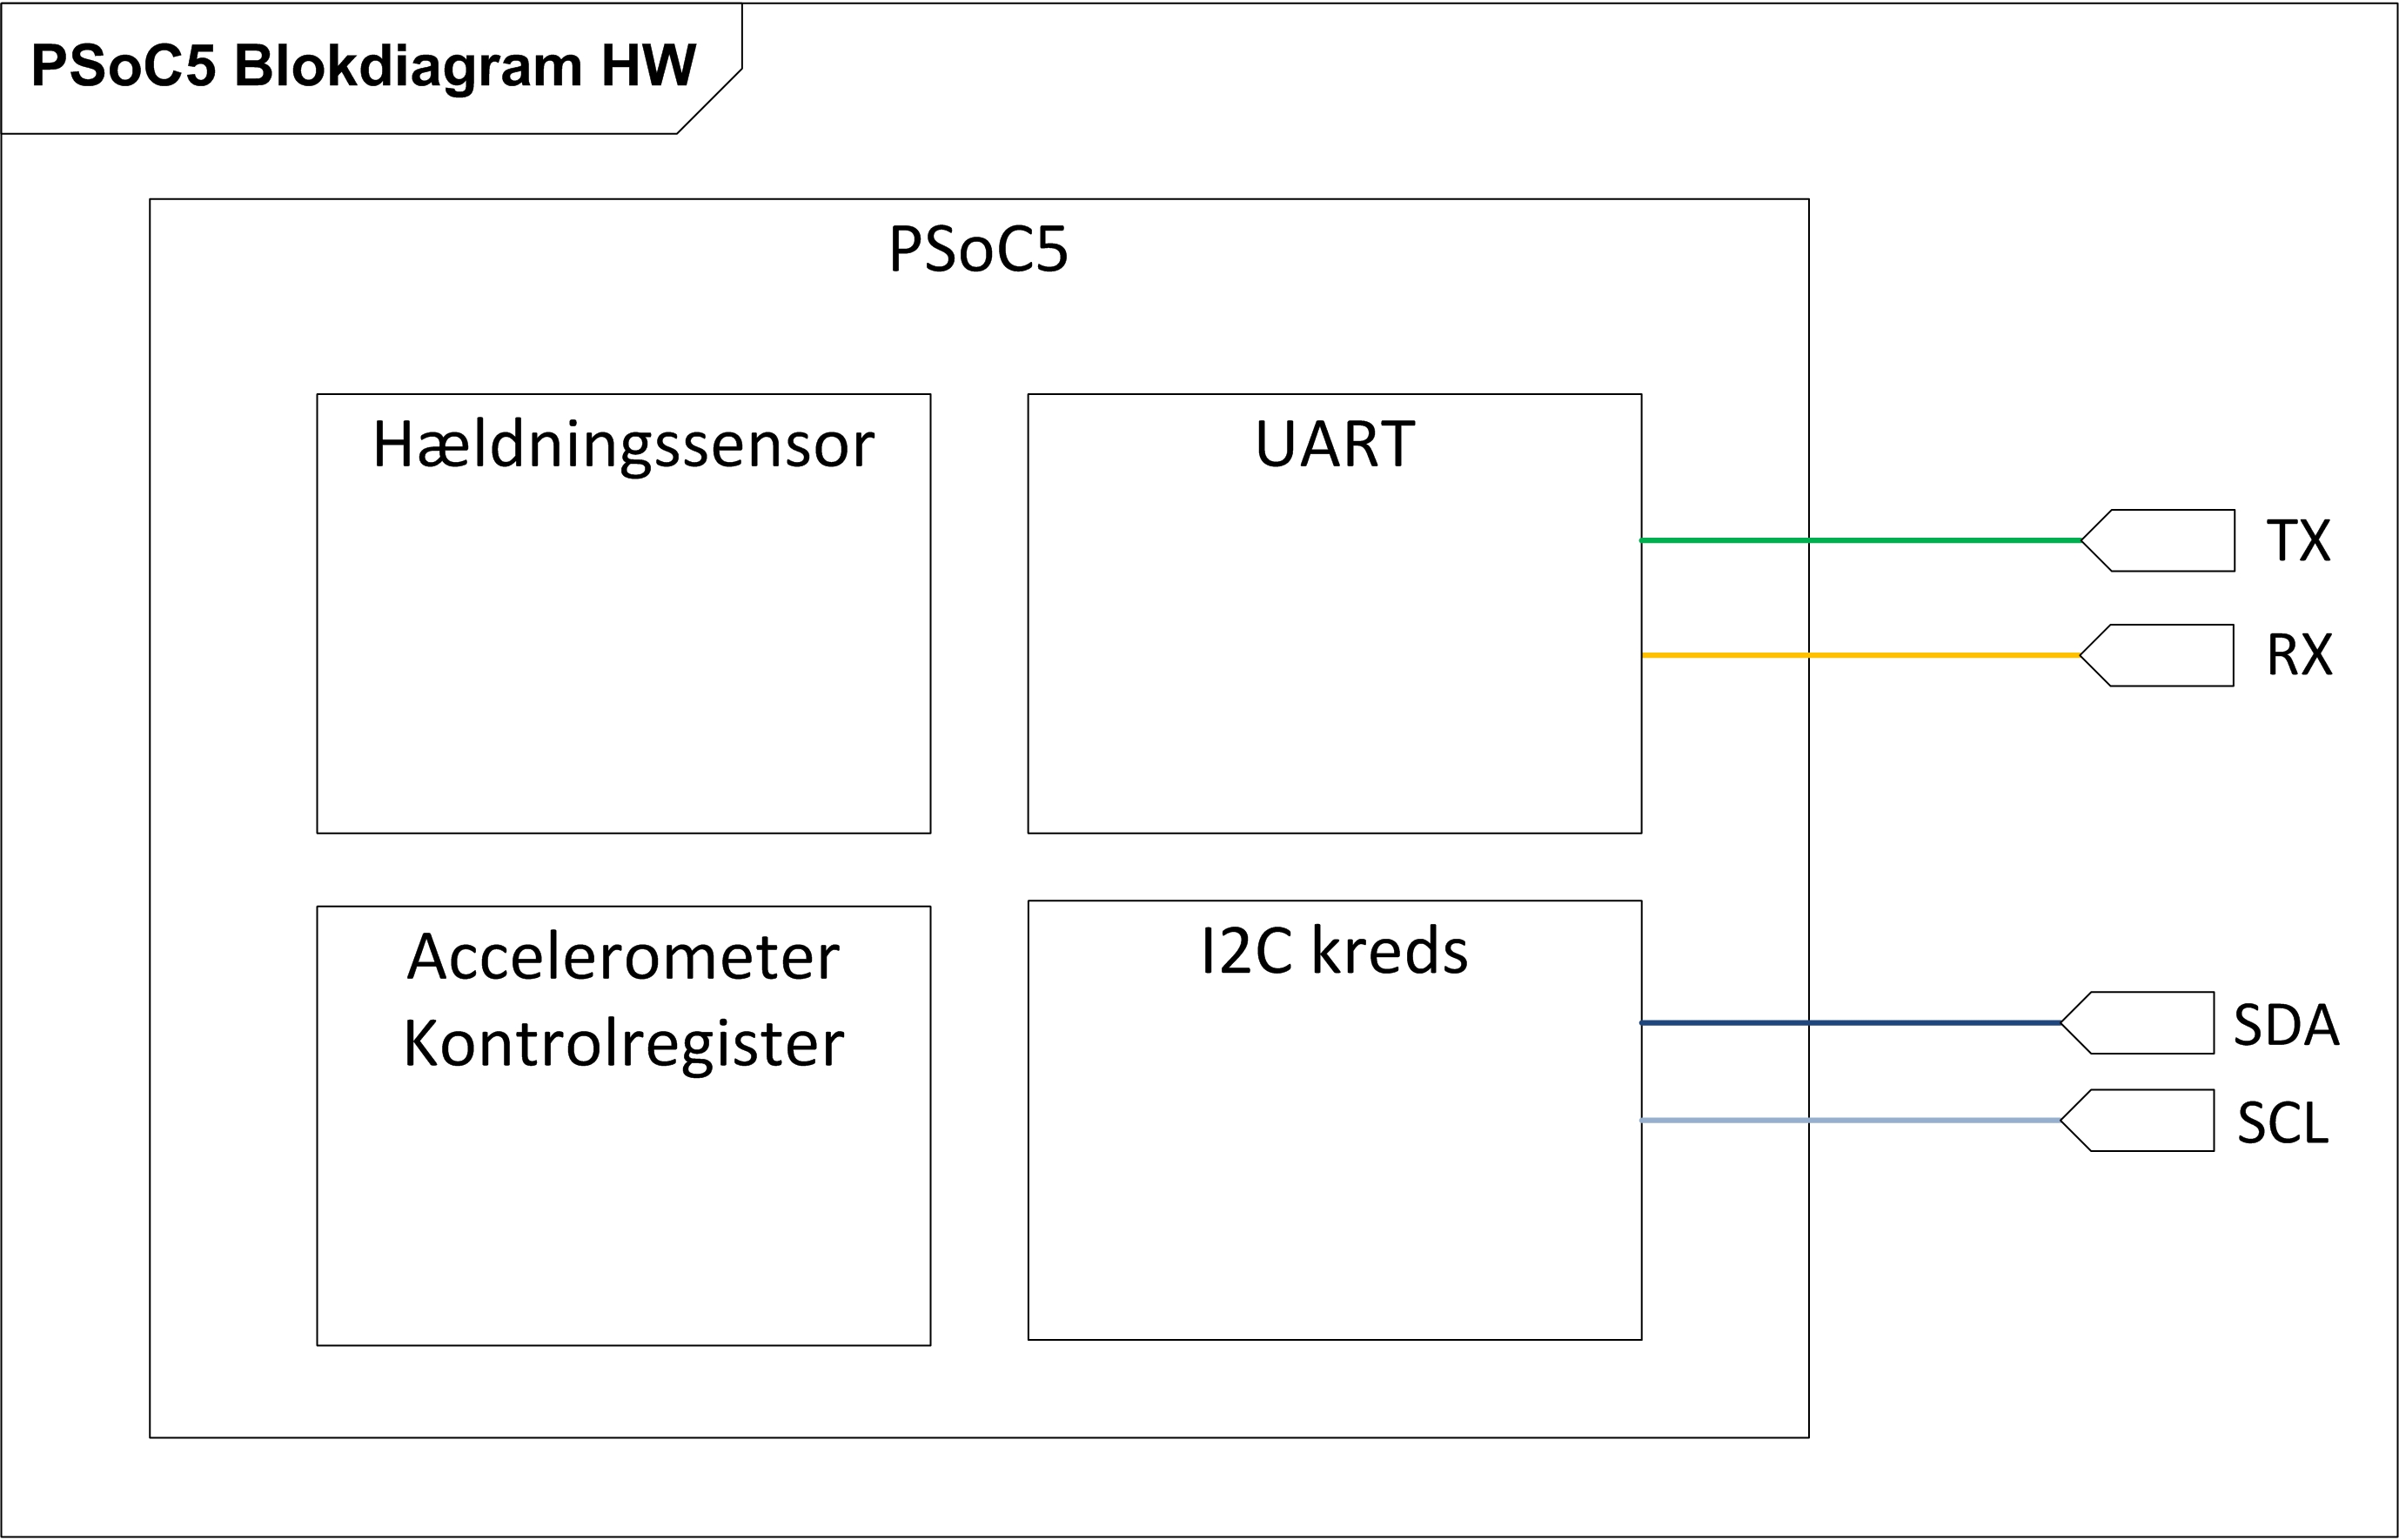
\includegraphics[width=0.80\textwidth]{billeder/SMPSoCblock}
	\end{minipage}
	\begin{minipage}[t]{0.48\textwidth}
	\caption{Hardware blok for SM}
	\label{fig:SMHW1}
	\end{minipage}
	\begin{minipage}[t]{0.48\textwidth}
	\caption{PSoC blok for SM}
	\label{fig:SMPSOC1}
	\end{minipage}
\end{figure}
Hældningssensoren består af 2 komponenter: det førnævnte accelerometer samt en DelSig ADC internt i PSoC'en. Valget af accelerometer kommer af at have lavet en række prototyper der ikke mødte vores krav, hvilket accelerometeret i PSoC'en gjorde. Valget af ADC faldt på en DelSig da, den er meget støj immun grundet det indbyggede lavpas filter og har en høj opløsning. Valgte komponenter er illustret på \textit{figur~\ref{fig:levelsensor}}. ADC konverterer det analoge signal fra, en pin forbundet til, accelerometer til en digital værdi der så senere bliver anvendt i softwaren. For ADC og accelerometerets opsætning se da afsnit \ref{ch:DetajlDesign}~\textit{Detaljeret hardware design} i Bilag.
\begin{figure}[htbp]
	\centering
	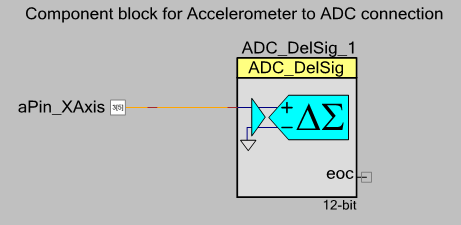
\includegraphics[scale=0.8]{billeder/levelsensor}
	\caption{Hældningssensorens implementering}
	\label{fig:levelsensor}
\end{figure}
\subsubsection{Software}
SM software behandler den konverterede data fra ADC'en samt kommunikation med VBTE og KI modulernerne. Sofwarens udvikling har fulgt de samme faser som hardwaren, hvilket har ført til letforståelig og læselig kode. Softwaren er illustreret på \textit{figur~\ref{fig:SMKD}}. Der vil efterfølgende blive taget udgangspunkt i et statemachine samt funktionen getFromKI.
\begin{figure}[H]
	\centering
	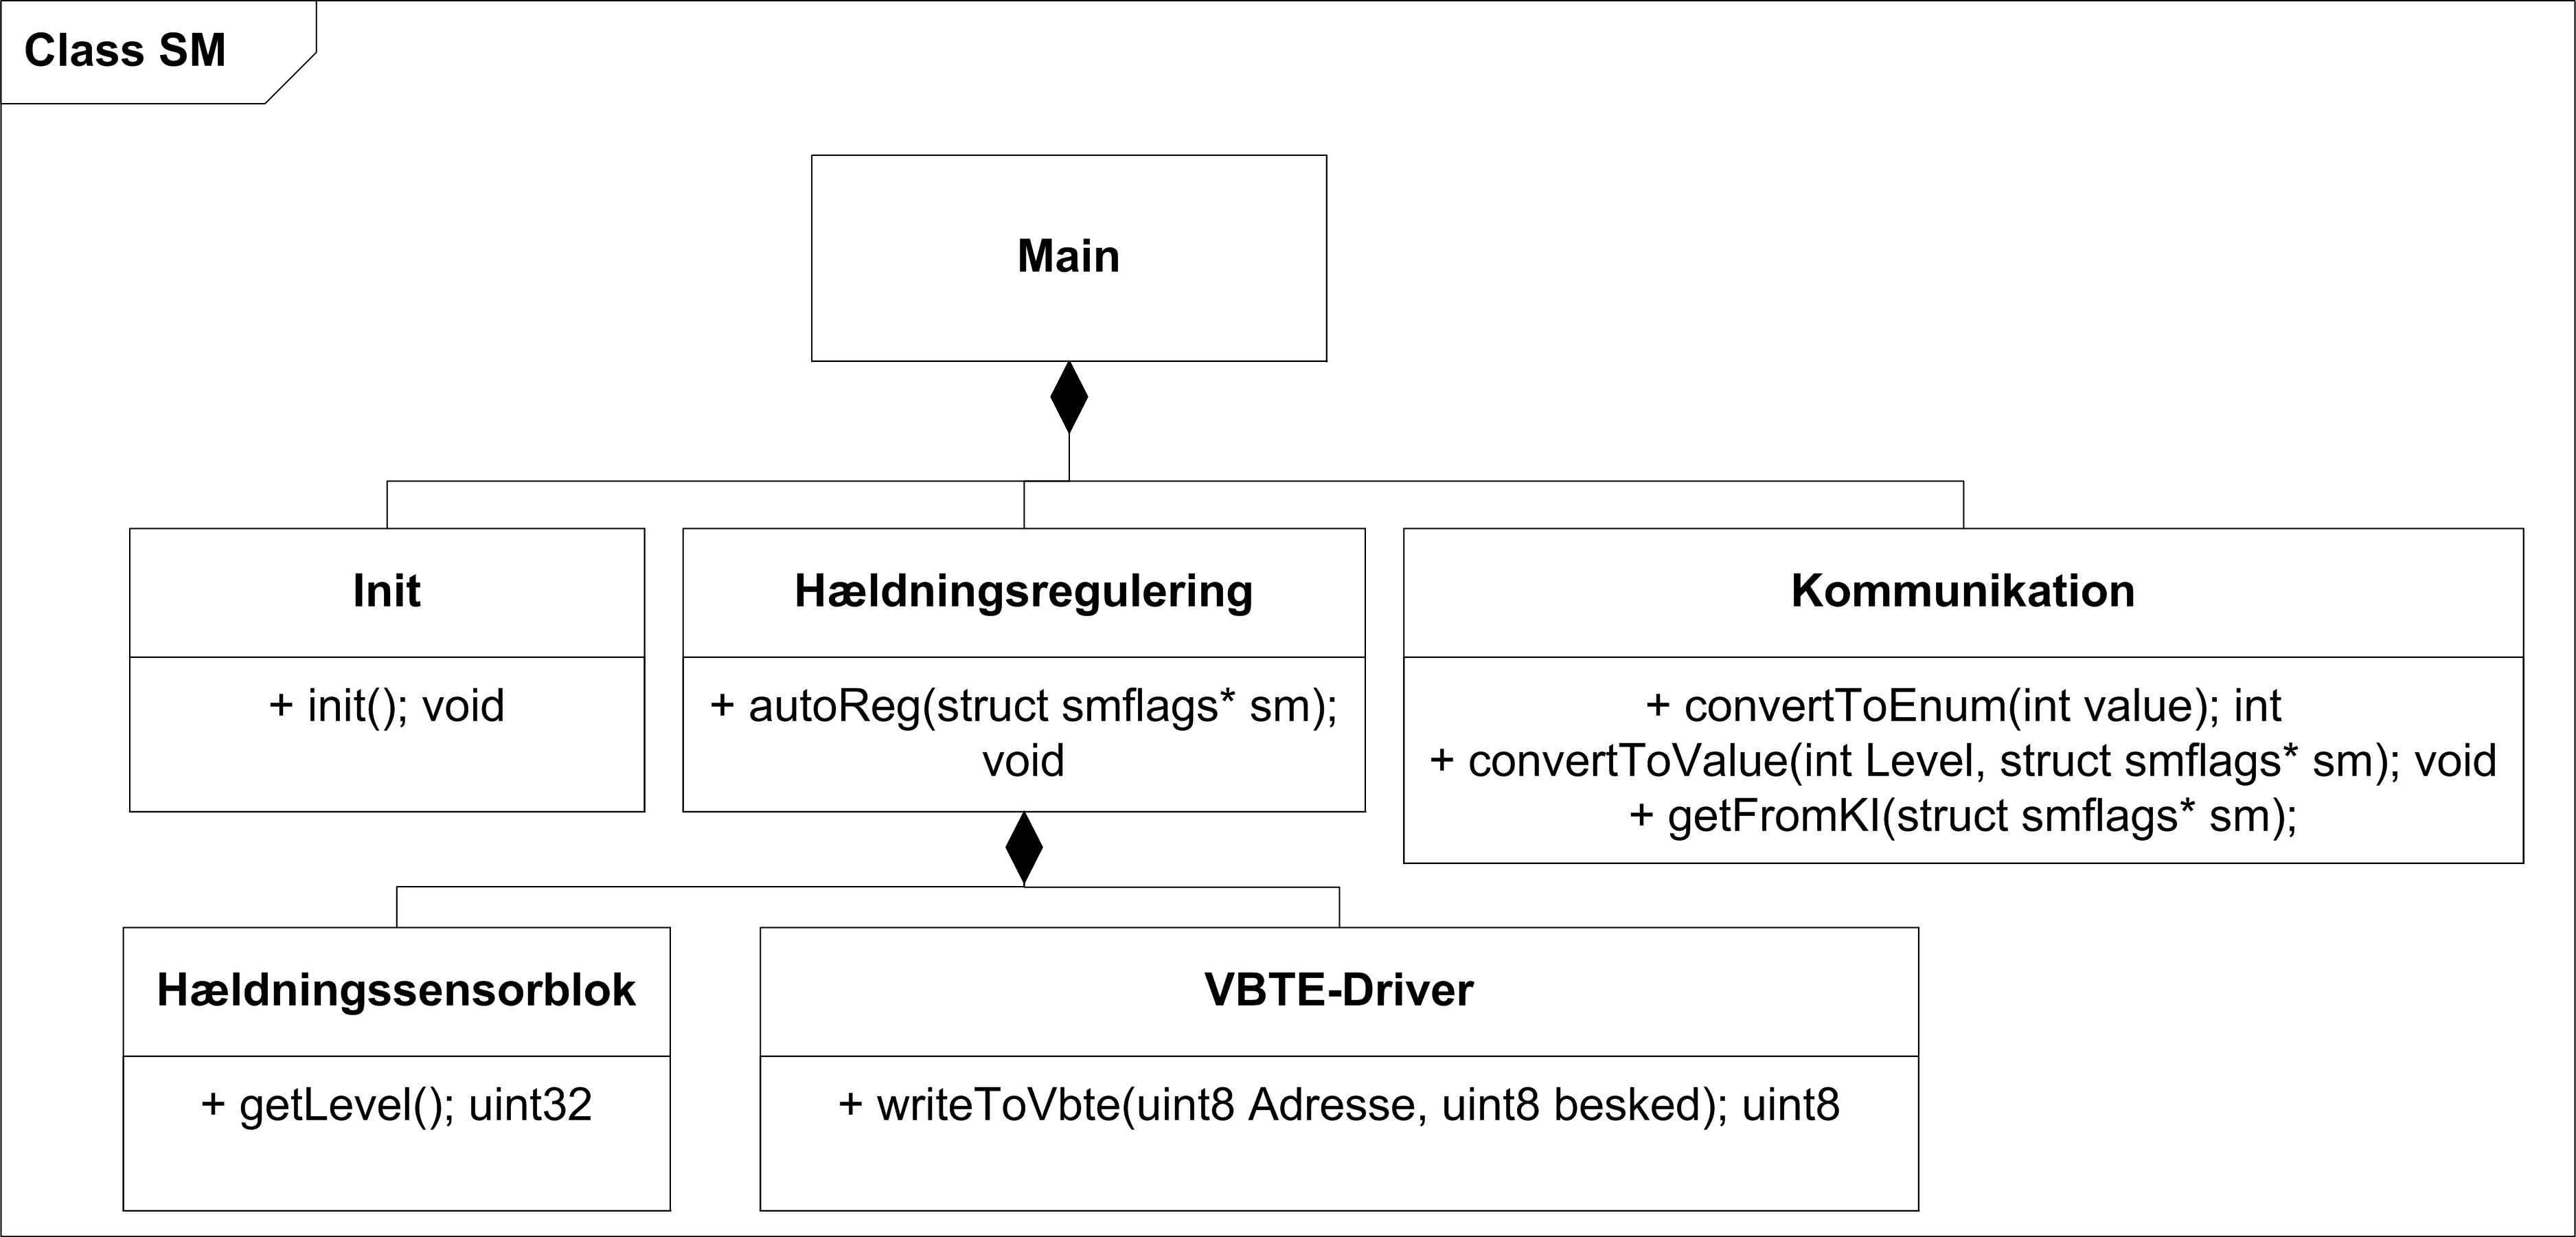
\includegraphics[width=0.75\textwidth]{billeder/smKlassediagram}
	\caption{Klassediagram for SM}
	\label{fig:SMKD}
\end{figure}
\textbf{SM funktionalitet}\\
Funktionalitet af SM kan bedst beskrives med et state diagram. På \textit{figur~\ref{fig:stm_sm}} ses  state machine diagrammet for SM modulet. Diagrammet indeholder hældningsregulering state der beskriver den automatiske og manuelle regulering i systemet. Den automatiske regulering styres med et flag. Den manuelle styres med en værdi der bliver sat. Flaget bliver sat når SM opnår forbindelse med KI modulet i 'Afvent' statet. Flaget bliver nulstillet hvis KI sender besked til SM modulet om at det skal termineres, hvorefter SM går tilbage i 'Afvent' statet. Behandlingen af beskeder fra KI i 'Modtag besked fra KI' og 'Send svar til KI' states ses i følgende afsnit \textit{getFromKI}.\\
\\
\textbf{getFromKI}\\
Funktionen er bedst beskrevet med et flowdiagram:
\begin{figure}[H]
	\centering
	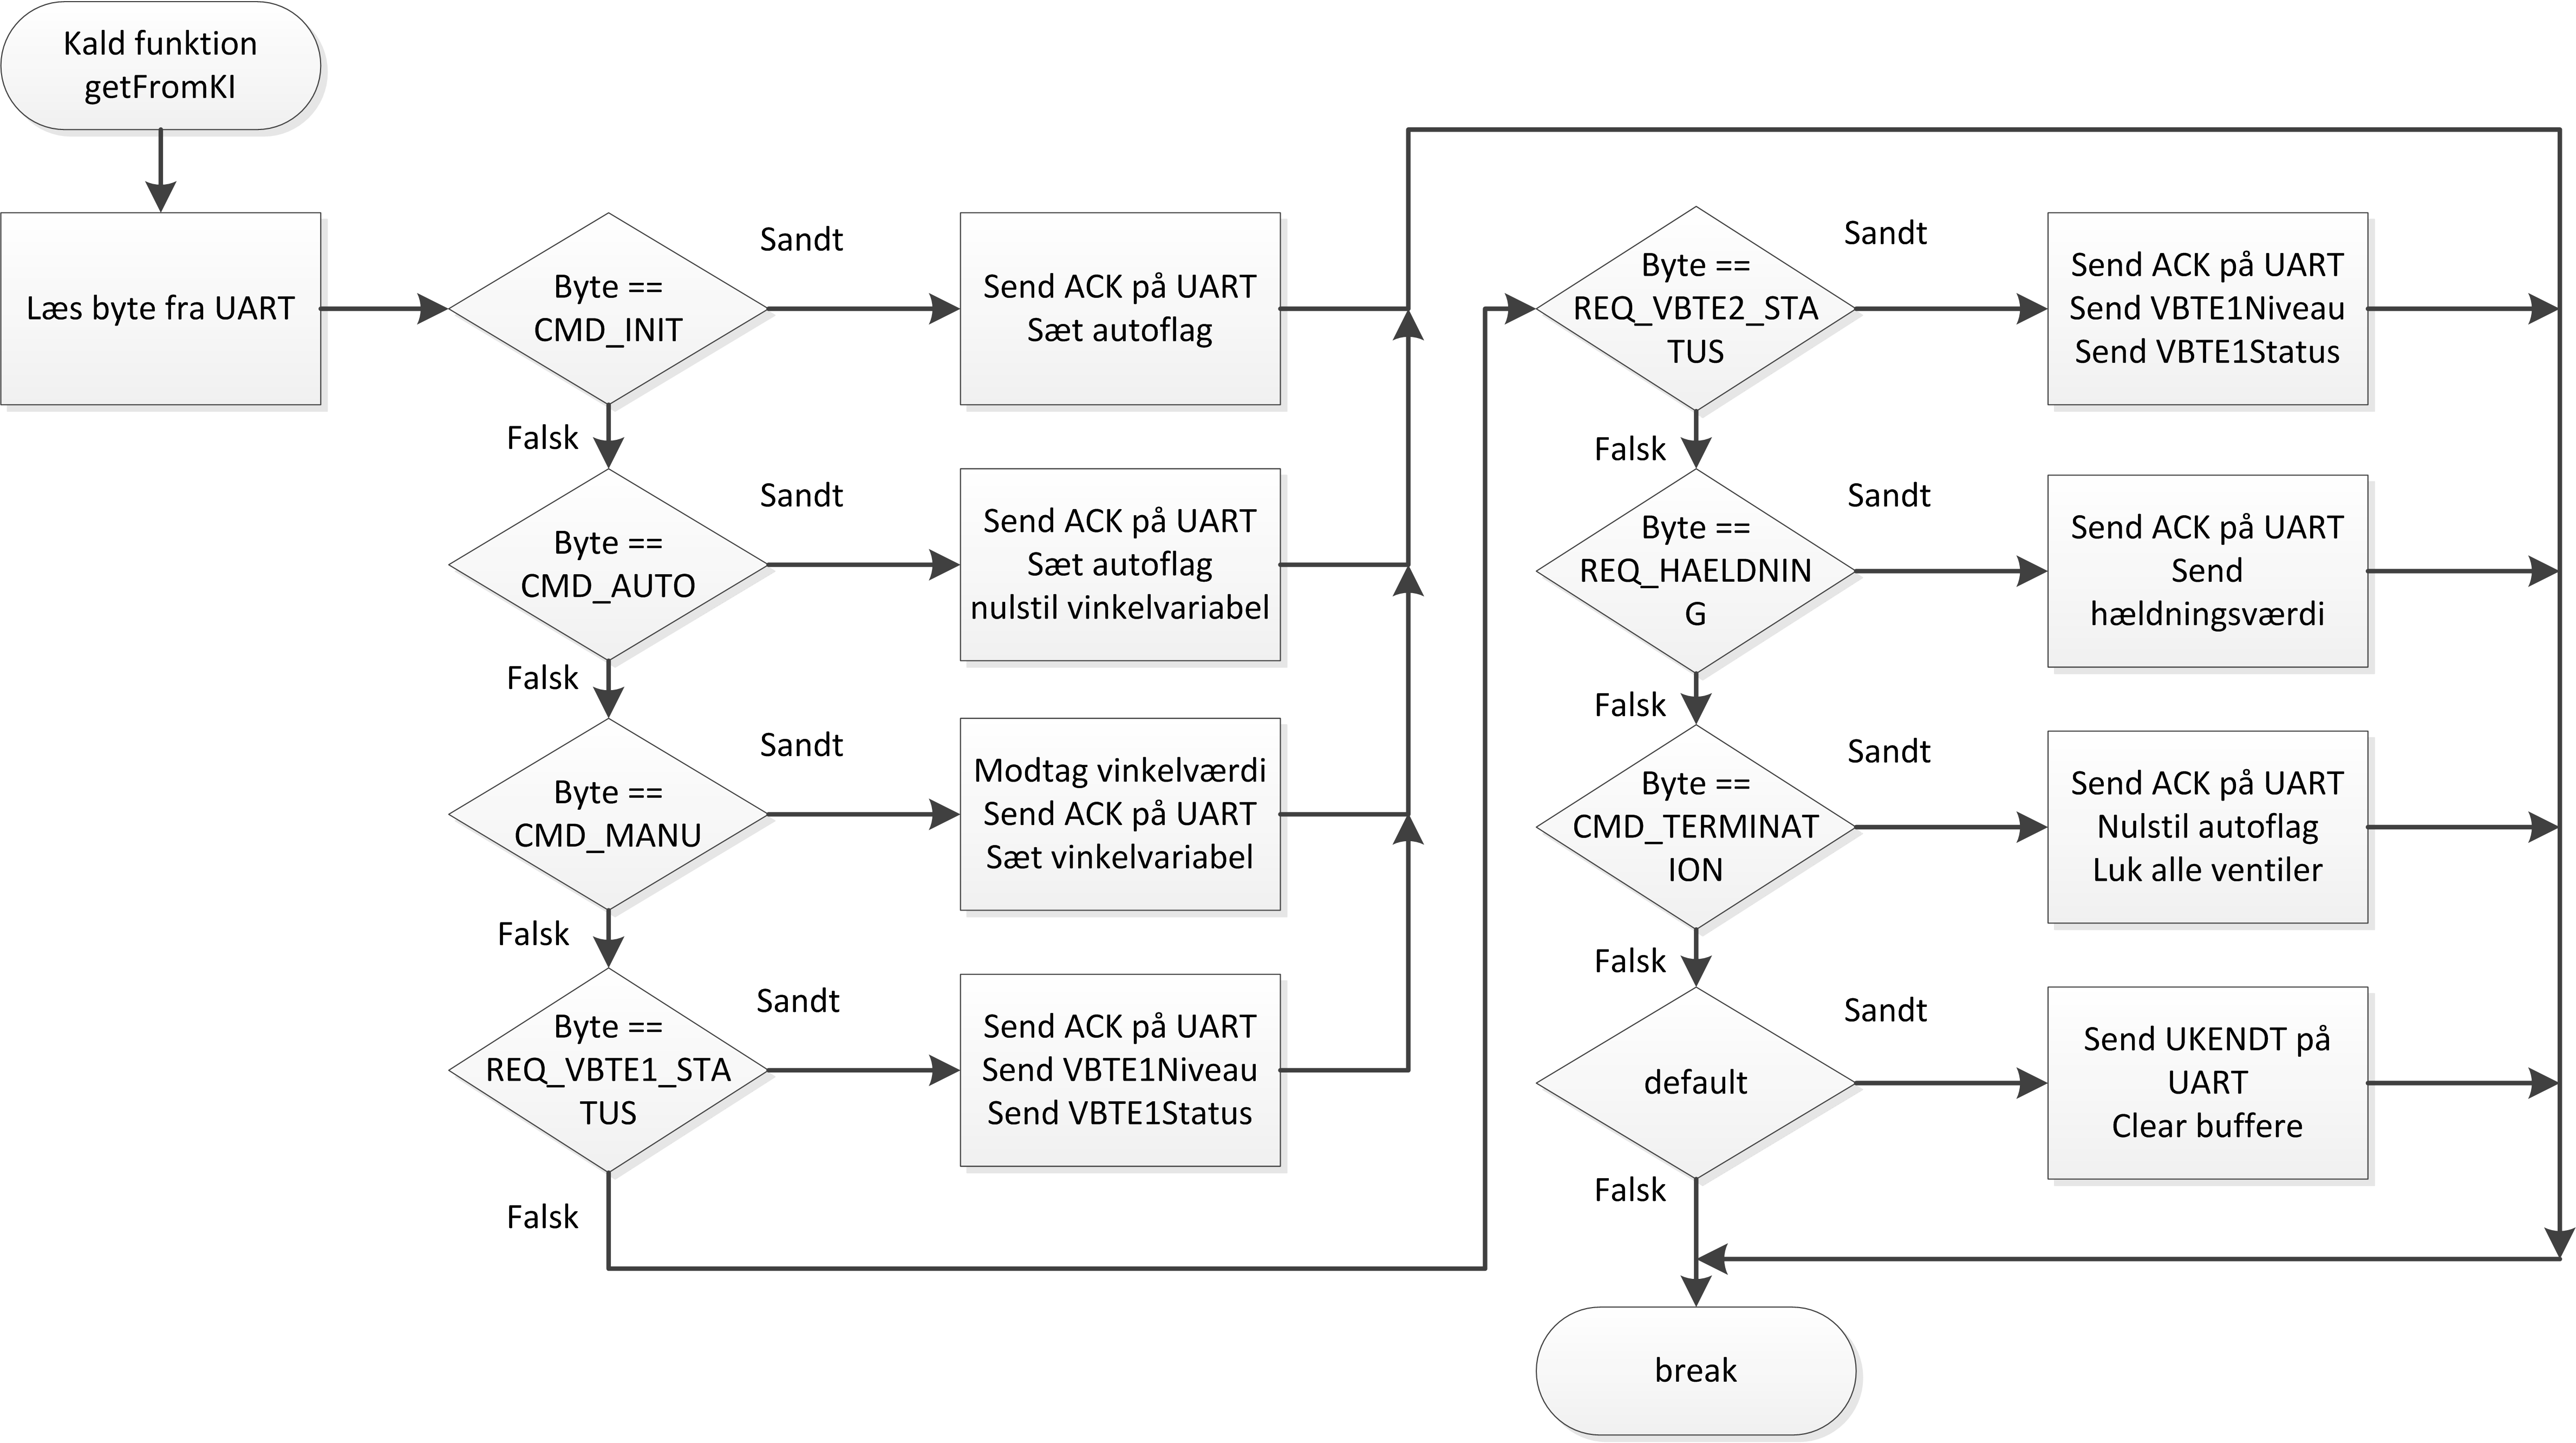
\includegraphics[width=0.75\textwidth]{billeder/getFromKIflowchart}
	\caption{Flowdiagram for funktionen getFromKI}
	\label{fig:gFKIfc}
\end{figure}
Funktionen har til ansvar at kommunikere med KI efter de krav opsat i Kravspecifikation. Hver ACK er relateret til den besked, der er modtaget, så KI modulet ved hvilken besked, SM har modtaget. Dette sikre pålidelig overførsel da KI modulet har mulighed for at validere på overførslen. getFromKI bliver kaldt ca. hver andet sekund for at se om KI har skrevet noget til bufferen. Hvis der ikke er noget i bufferen returnerer funktionen med det samme.\\
\subsection{Strømforsyning}
I dette afsnit beskrives design og implementering af strømforsying. Strømforsyningen implementeres sammen med SM og VBTE.
\subsubsection{Hardware}
Strømforsyning er designet til at levere to forsyningsspændinger: \textbf{12VDC 1A og 5VDC 0.5A} dette gøres fra en 24V AC forsyningskilde. 
For at gøre designet af strømforsyning mere oversskuelig er designfasen delt op i 3 faser:
\begin{enumerate}
\item Overordnet design
\item Nedbrydning af blokke
\item Opbygning af design
\end{enumerate}
Igennem de tre faser er designet af strømforsyning blevet udarbejdet, dette er gjort ved at have startet med et overordnet blokdiagram, hvor efter hver enkel blok er blevet beskevet og designet. \textit{figur \ref{fig:PowerSupplyBlok}} viser det overordnet blokdiagram af strømforsyningen.\\
\begin{figure}[H]
\centering
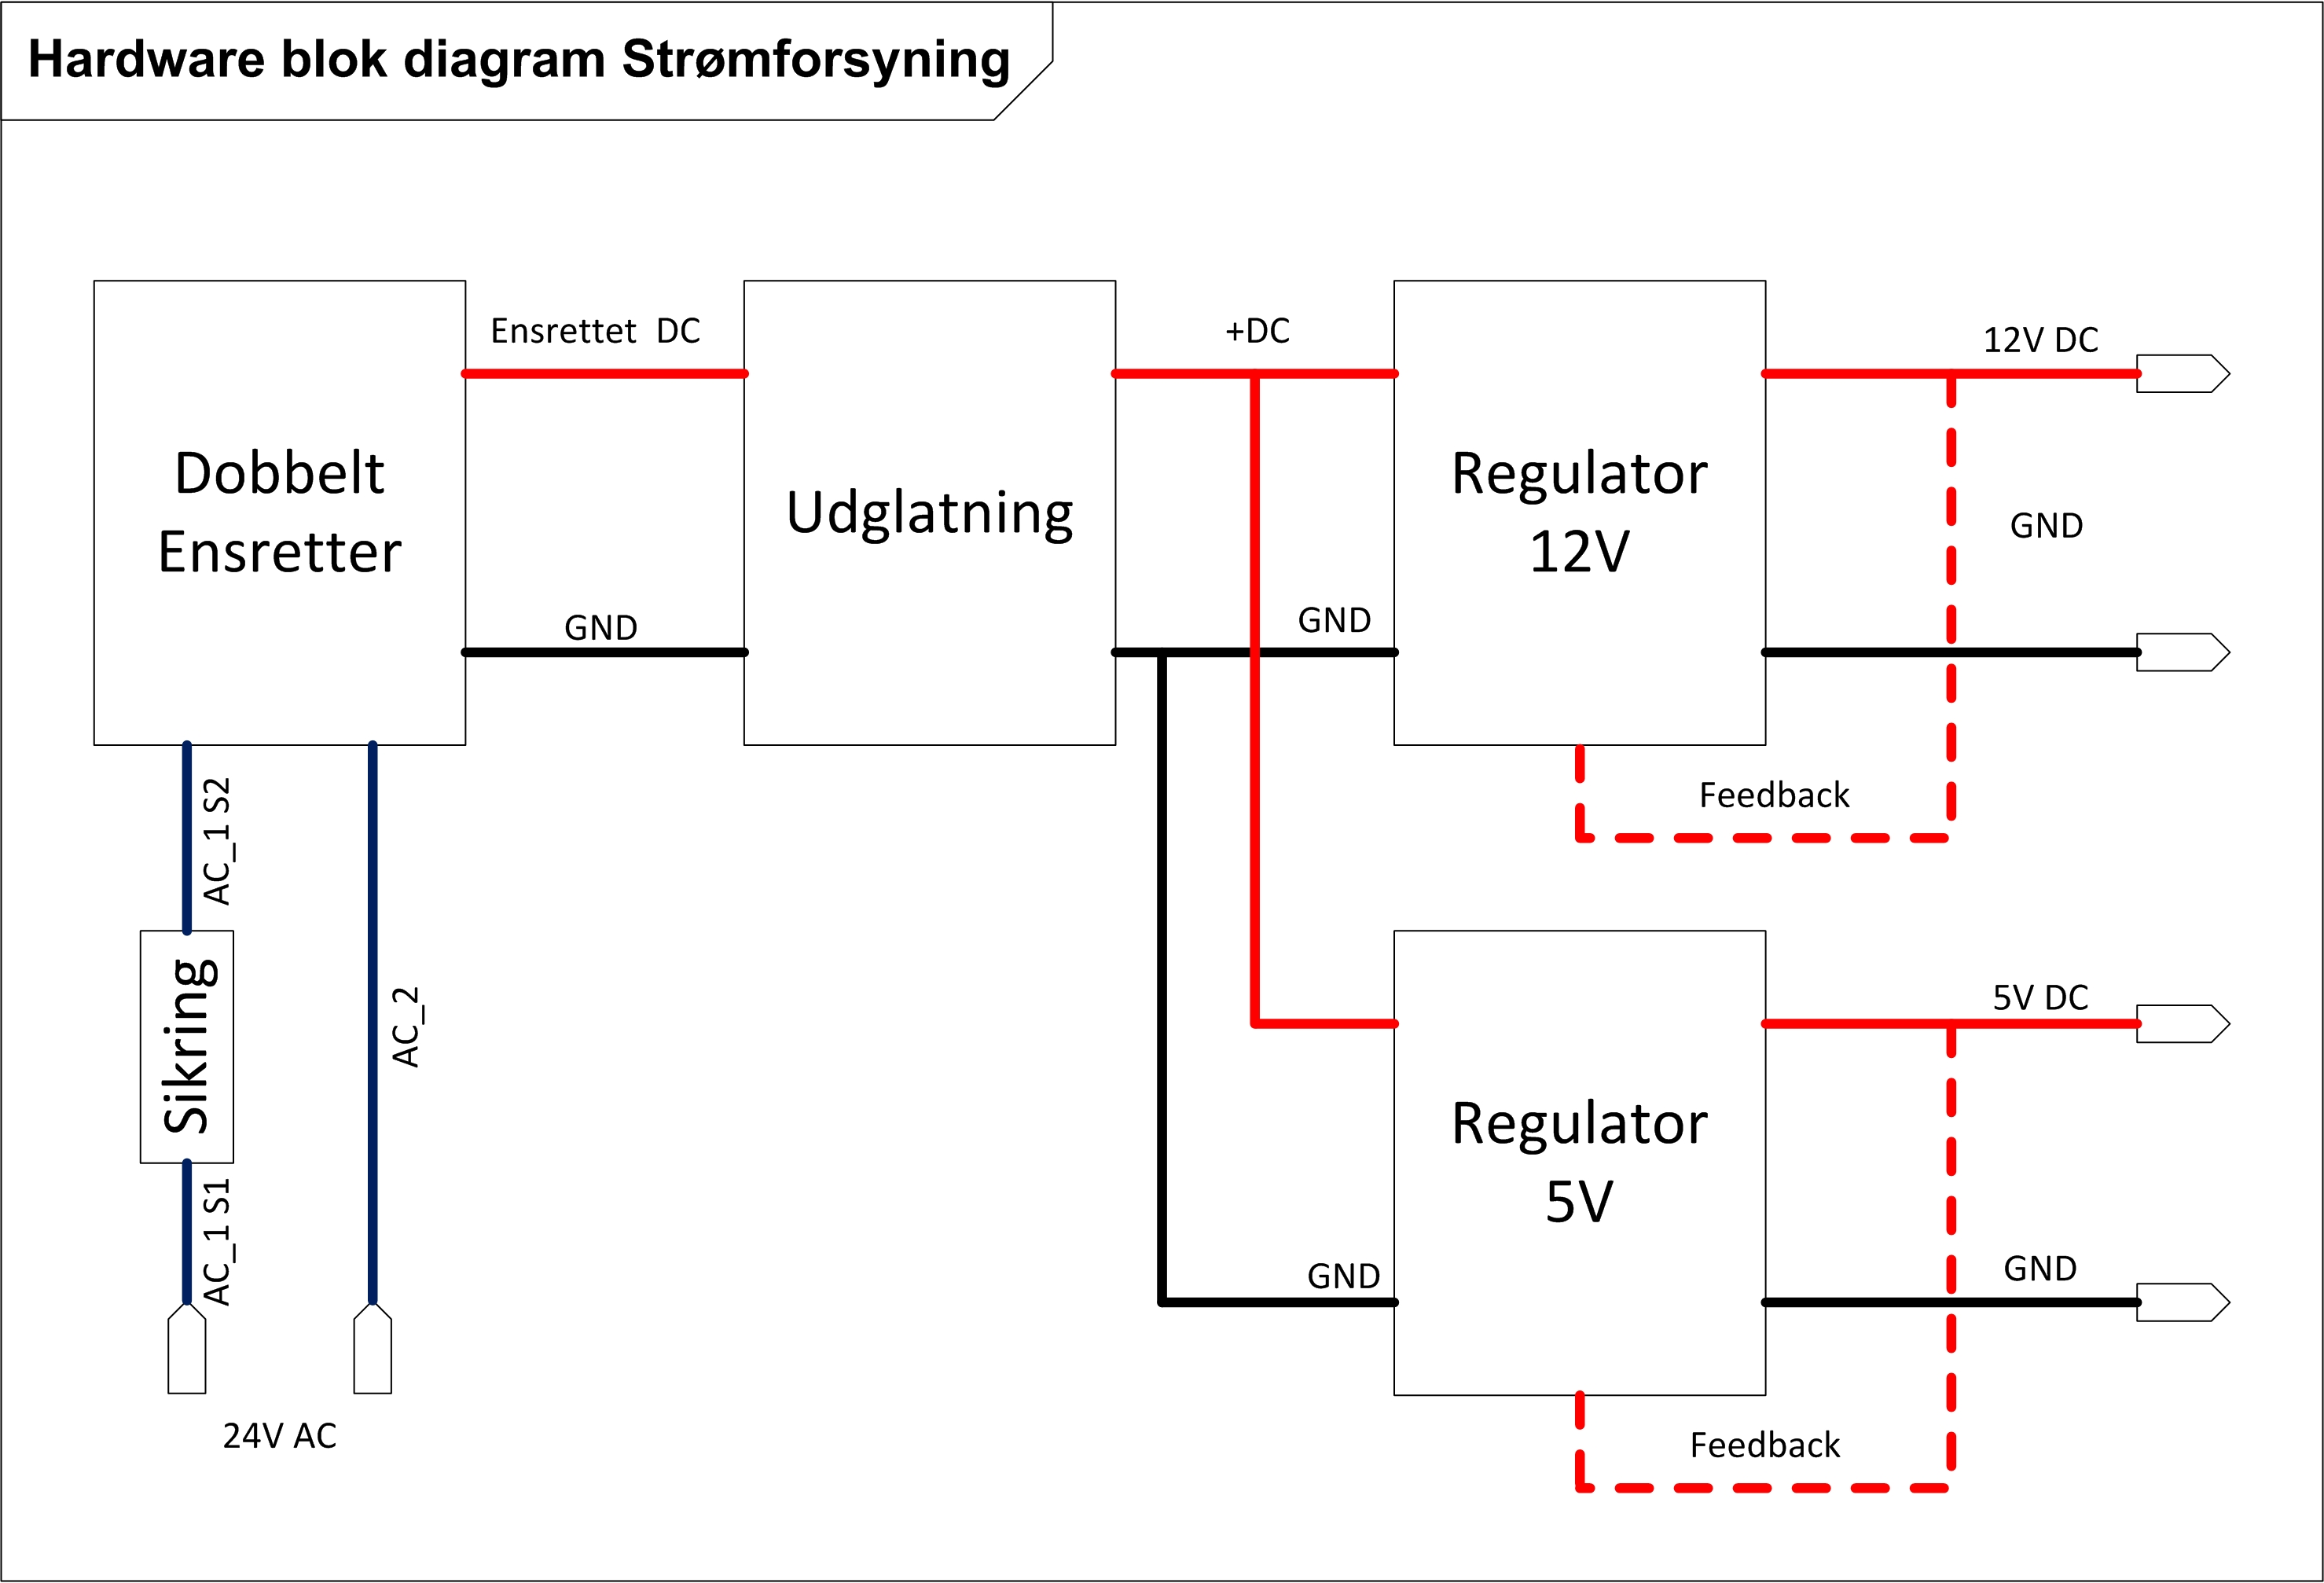
\includegraphics[scale=1]{billeder/PowerSupplyBlok}
\caption{Illustrering af overordnet blokdiagram af strømforsyningen.}
\label{fig:PowerSupplyBlok}
\end{figure}
\subsubsection{Beskrivelse af vitale hardware blokke}
I dette afsnit vil der være en beskrivelse af de udvalgte blokke.
\subsubsection{Dobbelt ensretter og udglatning}
Da strømforsyningen for leveret strøm fra en AC spændingskilde, skal AC signalet ensrettes til DC, dette gøres med dobbelt ensretter blokken og udglatnings blokken. 
\subsubsection{Dobbelt ensretter}
\begin{figure}[H]
\centering
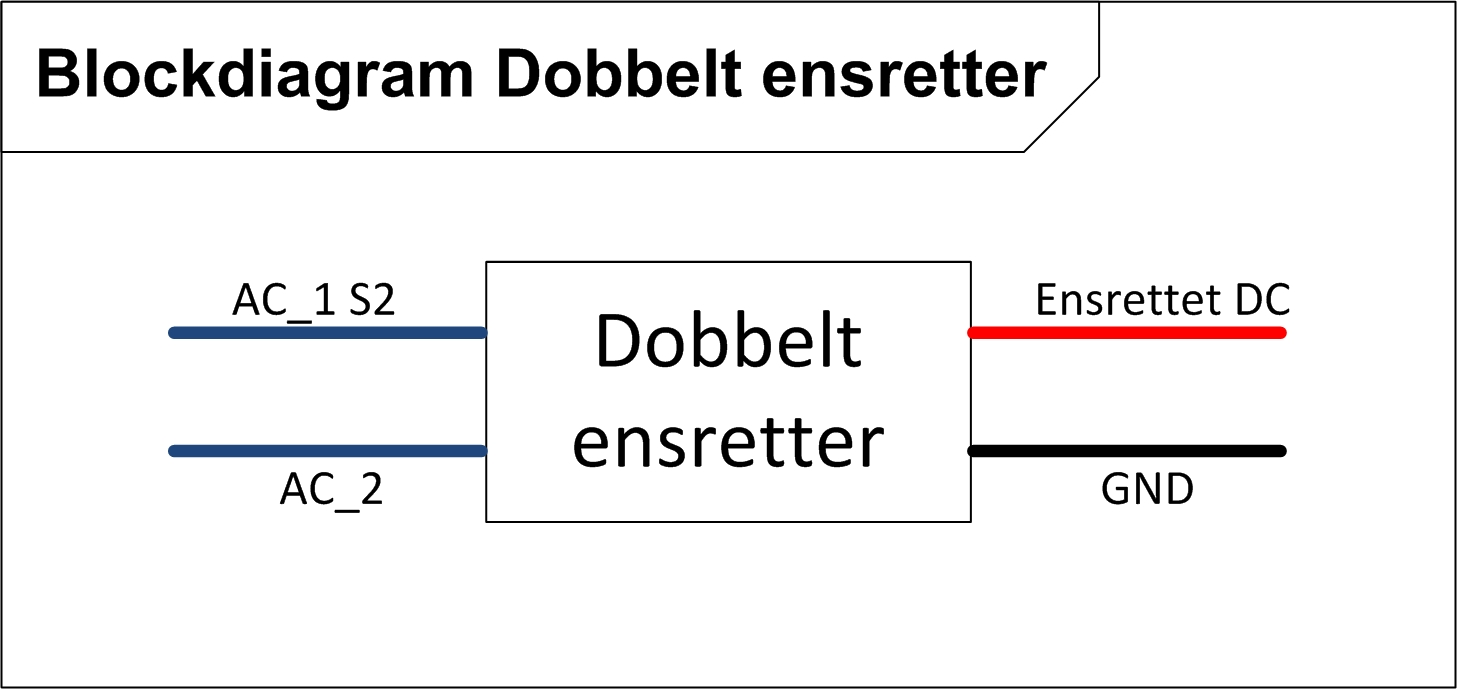
\includegraphics[scale=1]{billeder/DobbeltensretterBlok}
\caption{Blok for dobbelt ensretter}
\label{fig:DobbeltensretterBlok1}
\end{figure}
Dobbelt ensretteren en lavet som en diodebro bestående af 4 dioder, hvor to af dioderne samtiddig, hvilket betyder at der vil være positive halvperioder på udgangen "ensrettet DC" med en spidsværdi på ca. indgangsspænding * $\sqrt{2}$
\subsubsection{Udglatning}
\begin{figure}[H]
\centering
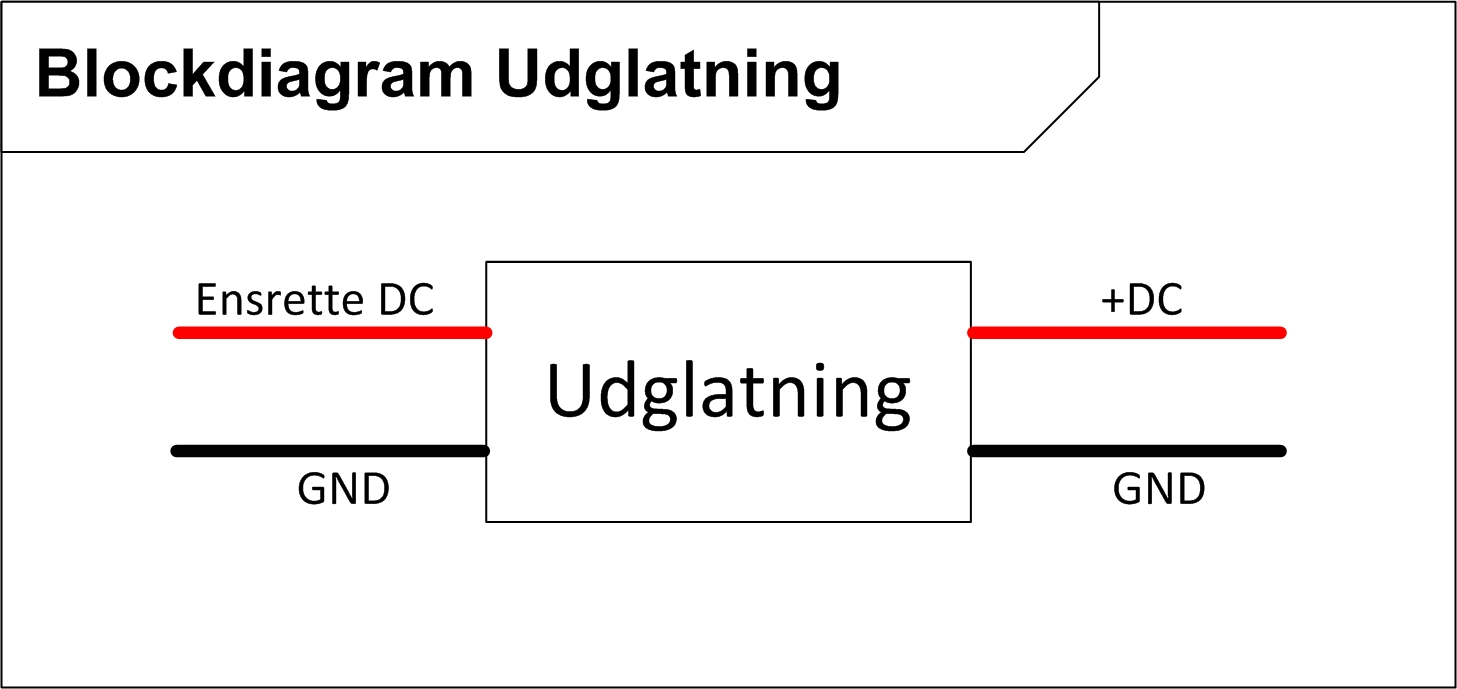
\includegraphics[scale=1]{billeder/UdglatningsBlok}
\caption{Blok for dobbelt ensretter}
\label{fig:DobbeltensretterBlok2}
\end{figure}
Udglatningen er en elektrolyt kondensator som oplades og aflades i forhold til de positive halvperioder, da kondensator kun når at aflade lidt for hver nedadgående periode, vil der være en jævn og stabil DC.  
\subsubsection{Regulator 12V og Regulator 5V}
Da de enkle moduler bruger 12V og/eller 5V skal DC spænding fra Udglatningen reguleres ned til det pasende niveau, dette gøres i blokkene regulator 12V og regulator 5V.
\begin{figure}[H]
	\centering
	\begin{minipage}[b]{0.48\textwidth}\centering
	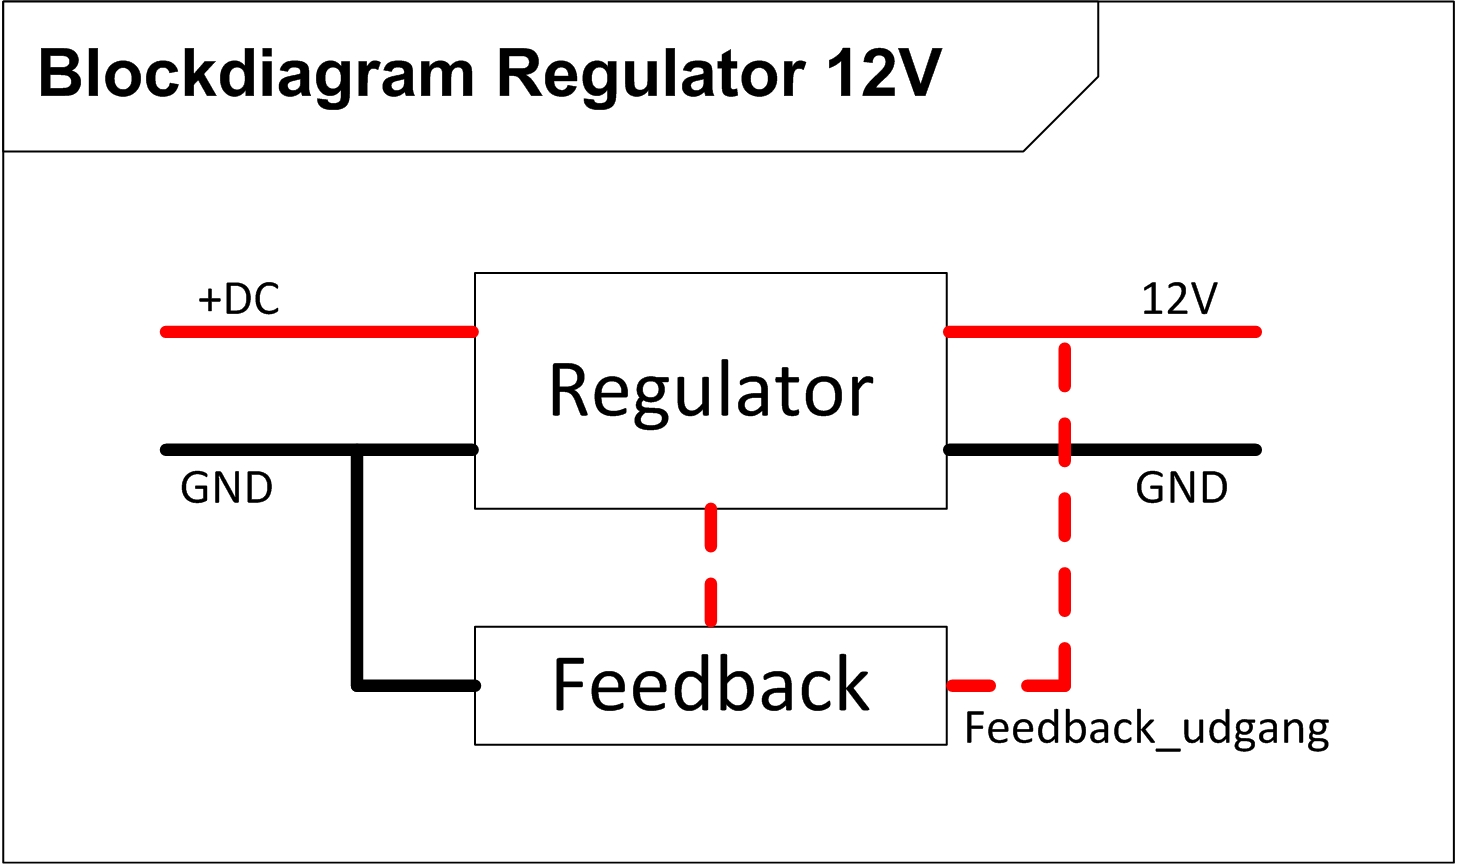
\includegraphics[width=0.80\textwidth]{billeder/Regulering_12VBlok}
	\end{minipage}
	\begin{minipage}[b]{0.48\textwidth}\centering
	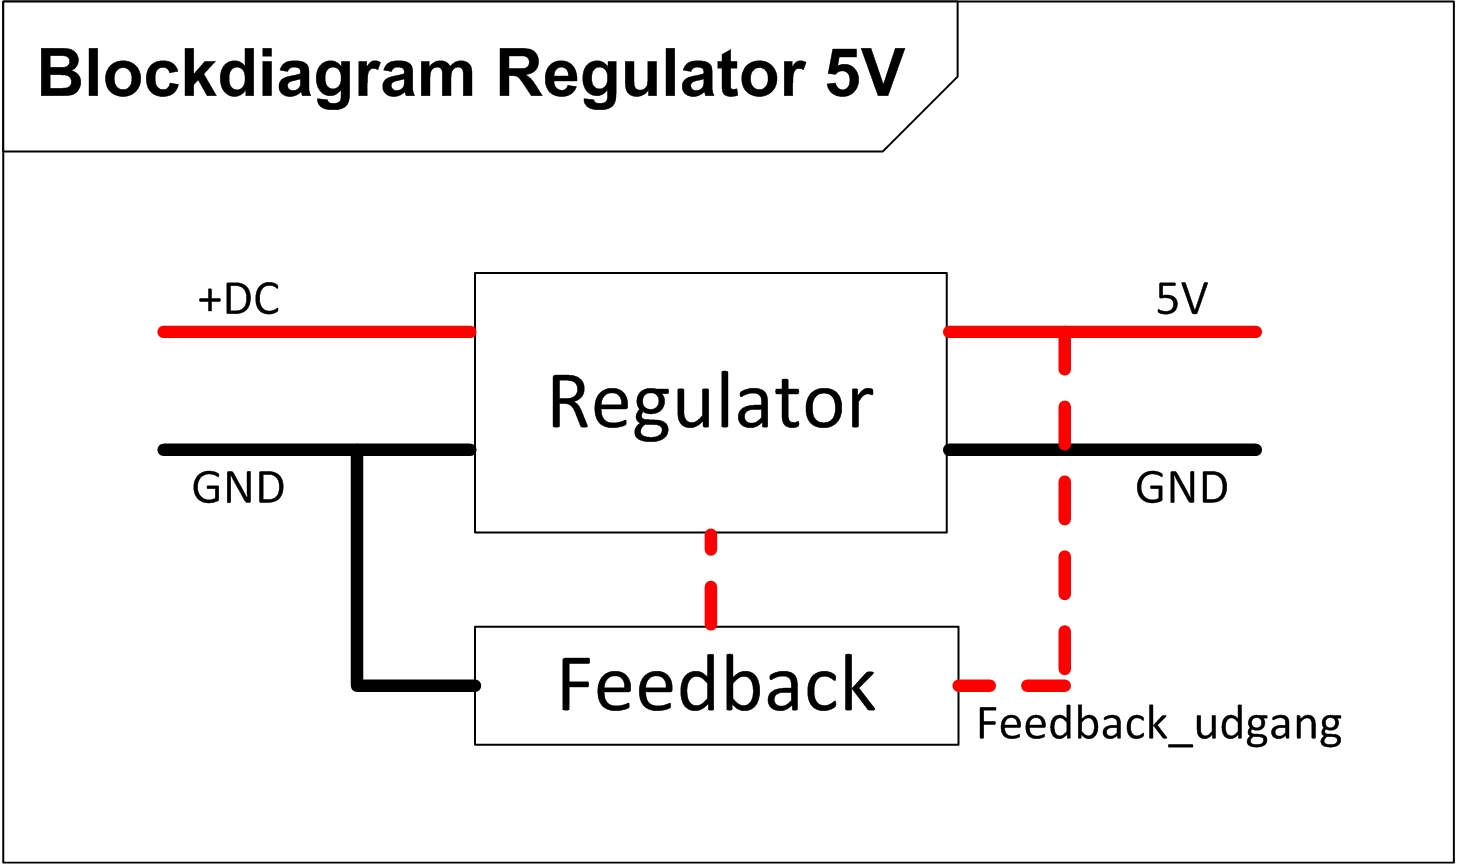
\includegraphics[width=0.80\textwidth]{billeder/Regulering_5VBlok}
	\end{minipage}
	\begin{minipage}[t]{0.48\textwidth}
	\caption{Blok for 12V regulator}
	\label{fig:Regulering_12VBlok}
	\end{minipage}
	\begin{minipage}[t]{0.48\textwidth}
	\caption{Blok for 5V regulator}
	\label{fig:Regulering_5VBlok}
	\end{minipage}
	\end{figure}
For at regulatoren kan regulere spændingen ned til 12V og 5V, bruges et feedback fra udgangen, feedbacket er indstillet til 12V ved hjælp af to modstande. \\




%%%%%%%%%%%%%%%%%%%%%%%%%%%%
%%%%%%%% DA TAB ACE  %%%%%%%
%%%%%%%%%%%%%%%%%%%%%%%%%%%%
\subsection{Database}
Denne section beskriver design og implementering af database delen som er lavet på baggrund af kravspecifikationen og systemarkitekturen.\\
Databasen er blevet opdelt i 2 dele som håndtere denne side. Databasen er opdelt i server og Webinterface.
\begin{figure}[H]
\centering
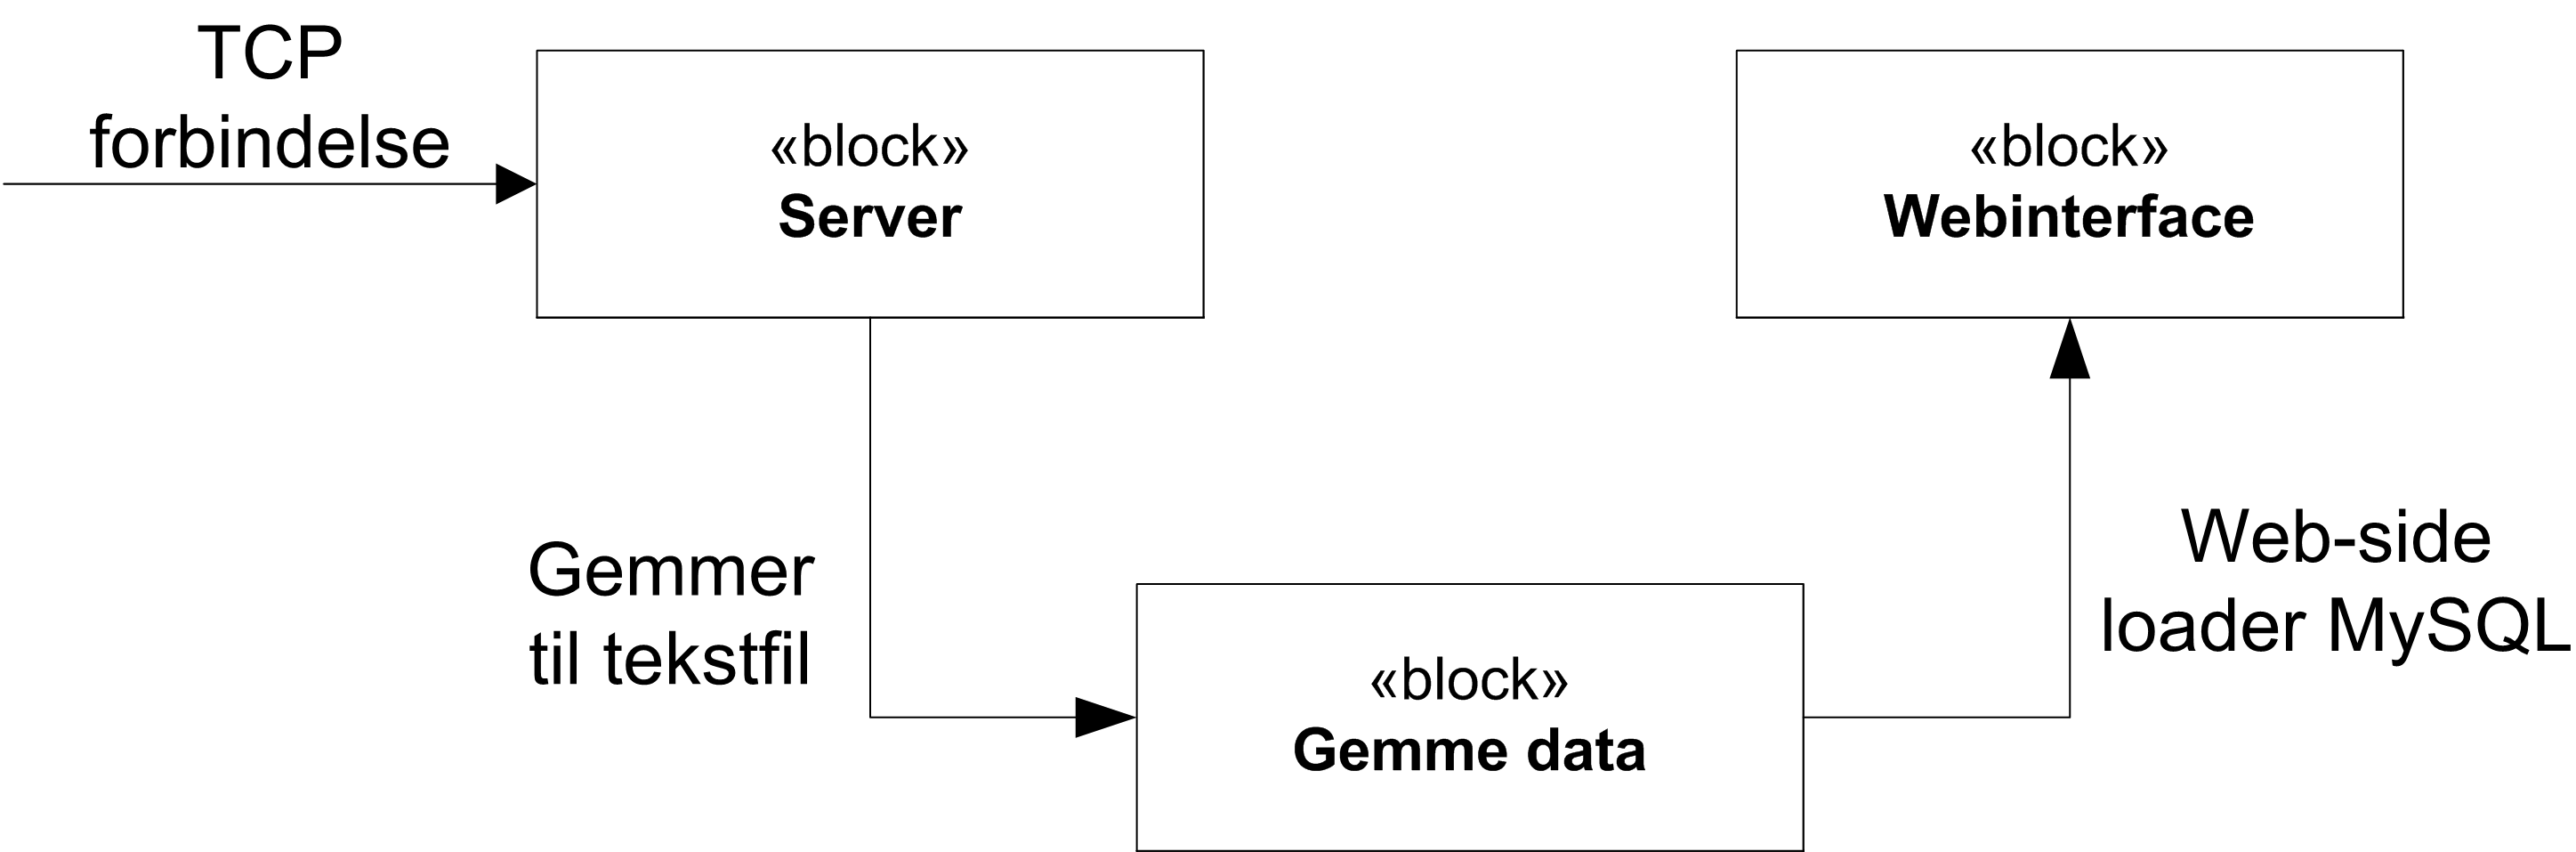
\includegraphics[width = 0.5\textwidth]{billeder/database_to_mysql}
\caption{Illustrere overordnet hvordan databasen fungere}
\label{fig:server_to_mysql}
\end{figure}

\subsection{Serveren}
Denne section beskriver design og implementering af serveren.
Opbygningen af serveren er gjort sådan at hver element i serveren er implementeret som en klasse, hvilket er illustreret på \textit{figur \ref{fig:database_server}}. For forståelse af det program flow der sker på serveren er der udarbejdet en statemachine \textit{figur \ref{fig:stm_server}} der hviser dette flow
\begin{figure}[H]
\centering
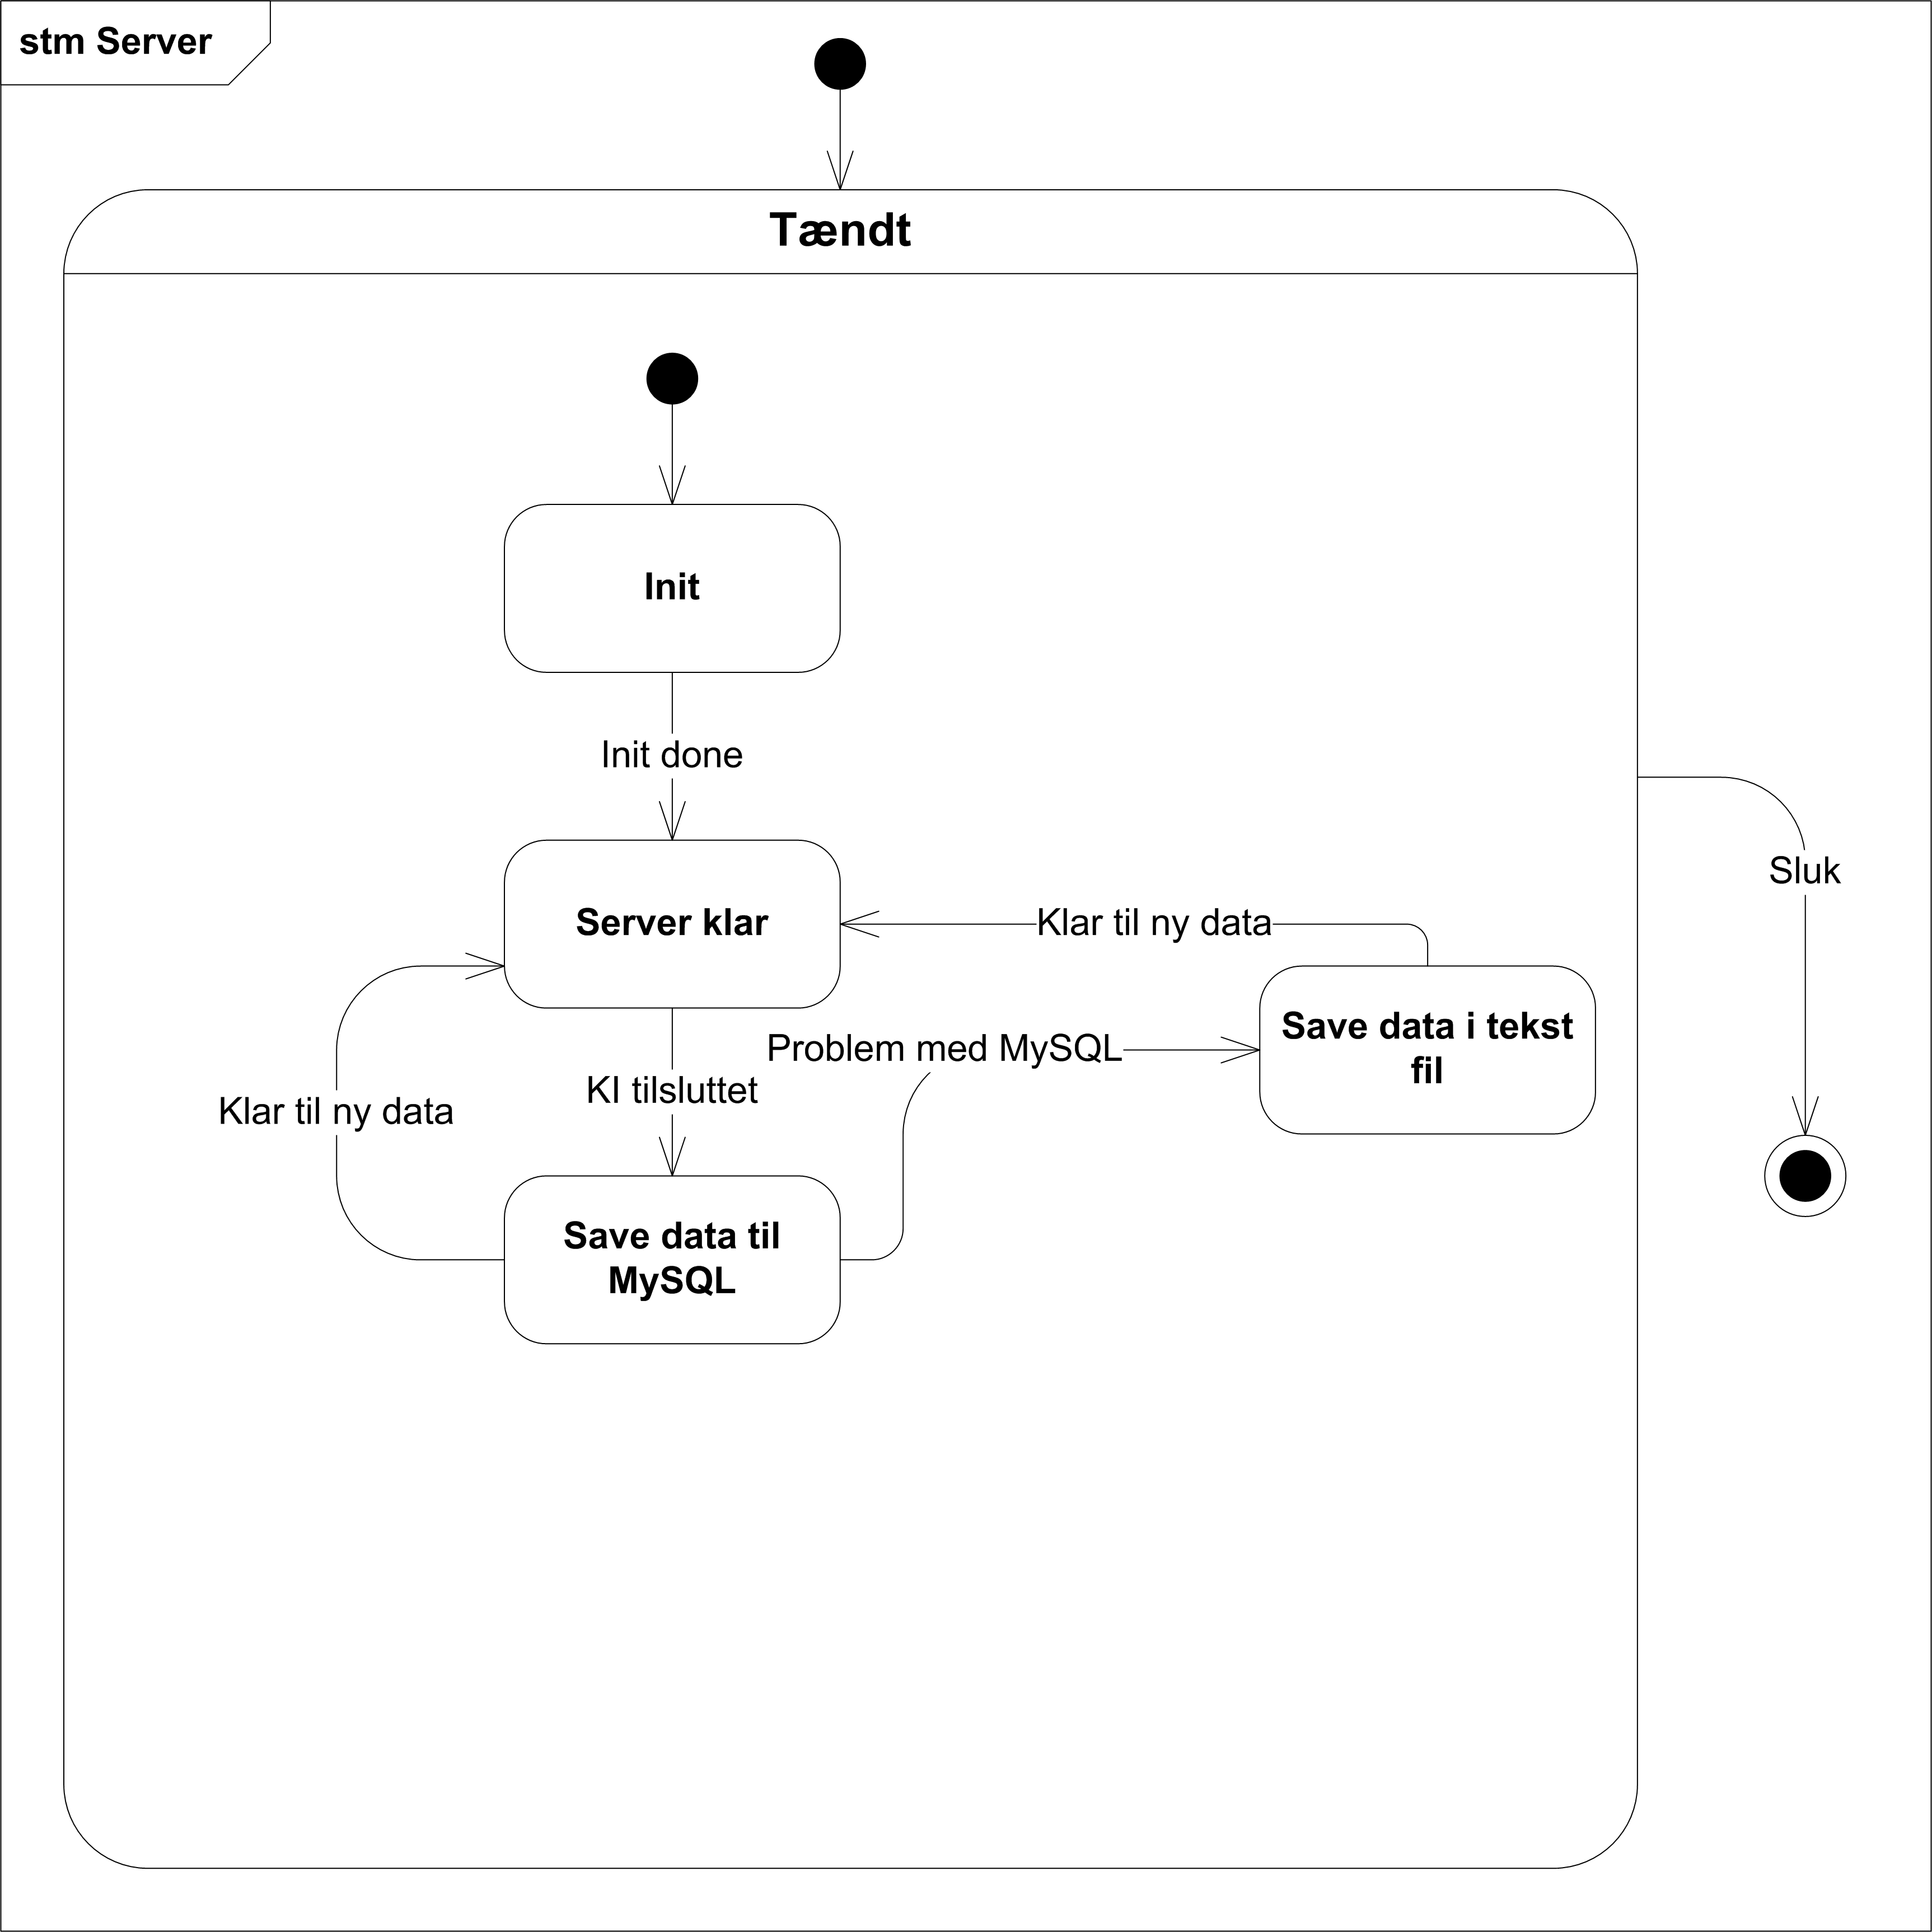
\includegraphics[width = 0.5\textwidth]{billeder/Systemarkitektur/stm_server}
\caption{Illustrere overordnet hvordan databasen fungere}
\label{fig:stm_server}
\end{figure}

Det gælder at når KI forsøger at kontakte databasen, tilsluttes denne via tcp som benytter sig af socket. Når tilslutningen er gjort kan der overføres data fra KI til databasen. Data bliver gemt i en tekst fil, der indlæses af Webinterface.
\begin{figure}[H]
\centering
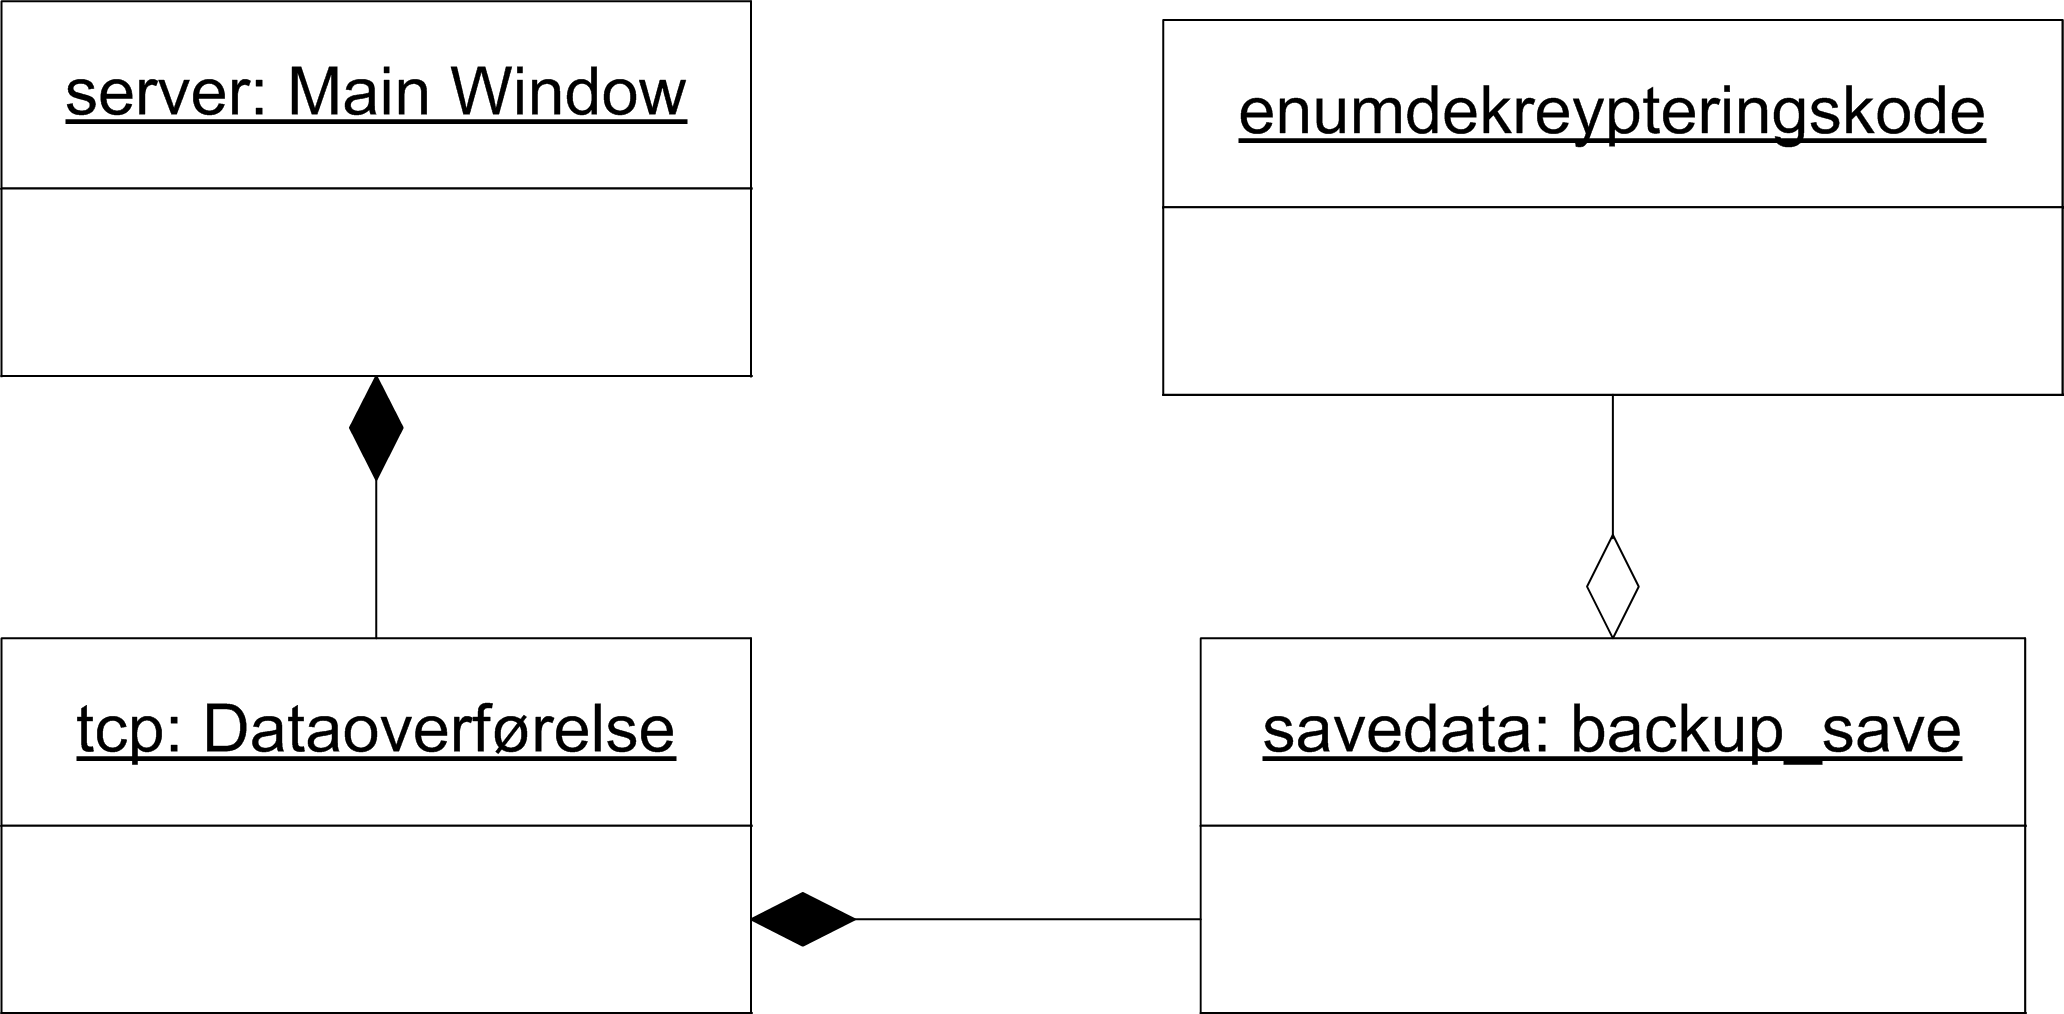
\includegraphics[width = 0.5\textwidth]{billeder/database_server}
\caption{Overordnet illustration af serveren funktionalitet}
\label{fig:database_server}
\end{figure}

\begin{table}[H]
\centering
\rowcolors{1}{white}{light-gray}
\begin{tabular}{| p{3cm}  p{12cm}|}
\multicolumn{2}{l}{{\Large Serverens klasser}} \\\hline

Server & Er hovedvinduet på serveren. Information til brugeren udskrives herfra og knapper er implementeret. \\\hline
TCP forbindelse (tcp) & Opretter en mulig tcp forbindelse hvor skibet kan tilslutte sig og overføre data.\\\hline
Gemme data (savedata) & Gemmer data til en tekst fil.\\\hline
De kryptering (enumDeKrypteringskode) & Dekryptere level fra sm så data bliver i grader\\\hline
\end{tabular}
\caption{Serverens klasser}
\label{tabel:server-klasser}
\end{table}

\section*{Hovedvindue for serveren}
Dette giver et kort billed på hvordan serverens funktion ser ud. Den fulde model kan ses i appendix
\begin{figure}[htbp]
	\centering
	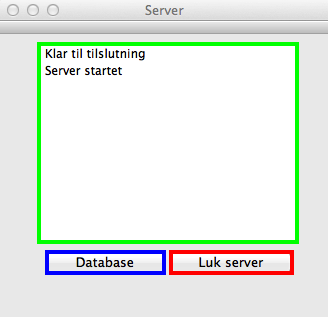
\includegraphics[width=0.4\textwidth]{billeder/server}
	\caption{Billed af serverens hovedvindue}
	\label{fig:server}
\end{figure}
Serverens GUI giver mulighed for at brugeren kan se at serveren køre og hvilke kommandoer der er blevet udført. Fra serverens hovedmodul har brugeren mulighed for at vælge at åbne den web baserede database. Der er en mulighed for at lukke serveren. Denne er ment som en mulighed for at lukke serveren i tilfælde af fejl eller restart da det er meningen at serveren skal køre konstant. Serverens grafiske visning er ikke til brug for terminaloperatøren men ment for at man kan se at serveren køre i stedet for at få udskrifter i terminalen.
\begin{table}[H]
\begin{tabular}{l p{12.5cm}}
\multicolumn{2}{l}{Hovedvinduets elementer} \\
\hline
\textcolor{green}{\textbf{1: Info}}
&Brugeren får her udskrevet beskeder om serveren. Brugeren kan se om KI har tilsluttet sig og om der er blevet overført data desuden vil fejl meddelelser blive udskrevet her. Dialog boksen er lavet sådan at den nyeste besked altid står øverst se \ref{fig:server}\\

\textcolor{blue}{\textbf{2: Database}}
&Anvendes til at lade brugeren tilgå den web baserede database. Efter log in og valg af skib komemr brugeren til databasen for skibet som ses i \ref{fig:database_web}\\

\textcolor{red}{\textbf{2: Luk serveren}}
&Anvendes til at lukke programmet. Bruges til nedlukning\\

\end{tabular}
\end{table}


\subsection{Webinterface}
Denne section beskriver design og implementering af web siden.\\
Opbygningen af Webinterface er gjort i php hvor dette gav mening. Desuden er html og styles (css) blevet benyttet til at sikre ens stil på hele web siden og for simpelt at kunne veligeholdes. For at sikre mindst data transmision imellem computer og server er princippet i ajax blevet benyttet.
Til at fremvise et grafisk program flow benyttes der en statemaschine \textit{figur \ref{fig:stm_web}}
 
\begin{figure}[H]
\centering
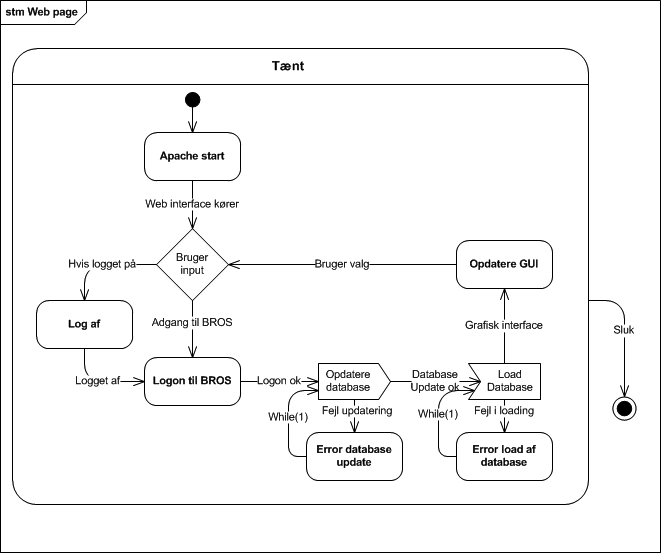
\includegraphics[width = 0.5\textwidth]{billeder/Systemarkitektur/stm_web}
\caption{Illustrere overordnet hvordan databasen fungere}
\label{fig:stm_web}
\end{figure}

Når havneterminalen ønsker at se data om skibe der er opkoblet på BROS kan denne tilgå disse via den web baserede database. Når serveren køre kan brugeren tilgå databasen via knappen "Database" ellers kan denne tilgås via ip adressen dette giver mulighed for at tilgå siden via internet hvorved at behovet for adgangskode ved log in er nødvendig for at sikre data imod uatorisret brug. Efter log ind på siden, kan brugeren vælge, hvilket skib der skal benyttes. Når skib er valgt kommer brugeren ind på den valgte database. Her kan brugeren se ID på skibet vandtilstand i ballast tanke, hældning og tid siden sidste opdatering (for nærmere se AppendixB). Webinterfacet checker hvert 5 secund om der er kommet ny data. Ved ny data vil et script sørge for at denne bliver gemt i MySQL databasen. Webinterfacet tilgår den angivne tabel i den angivne database. Til at håndtere wibinterfacet benyttes en apache server som er installeret på serveren. Apache serveren kan benyttes med de fleste operativ systemer.

\begin{figure}[H]
\centering
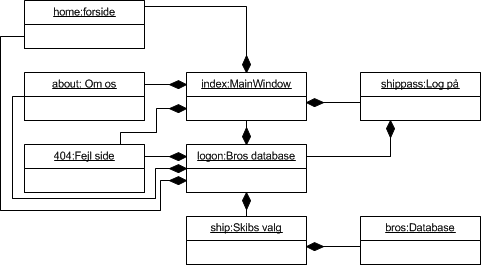
\includegraphics[width = 0.5\textwidth]{billeder/database_web}
\caption{Illustrere overordnet hvordan web-siden fungere}
\label{fig:database_web}
\end{figure}

\begin{table}[H]
\centering
\rowcolors{1}{white}{light-gray}
\begin{tabular}{| p{3cm}  p{12cm}|}
\multicolumn{2}{l}{{\Large Webinterface beskrivelse}} \\\hline
MainWindow \phantom{m}(index) & Index loader shippas ind som er en form som håndtere adgangskoder. Dette er siden brugeren kommer til som det første. Brugeren skal taste sin adgangskode for at få adgang til databasen\\\hline
Databasen  \phantom{m}(logon) & Denne side bliver kaldt efter at brugeren er logget på. Her vælger brugeren hvilket skib denne ønsker at få vidst data for.\\\hline
\end{tabular}
\caption{Web sidens opbygning}
\label{tabel:webside-simpel}
\end{table}

\subsection*{Skibs data i database}
Et billed af hvordan data fremvises for brugeren. For de andre sider på websitet kan disse ses i apendix
\begin{figure}[H]
	\centering
	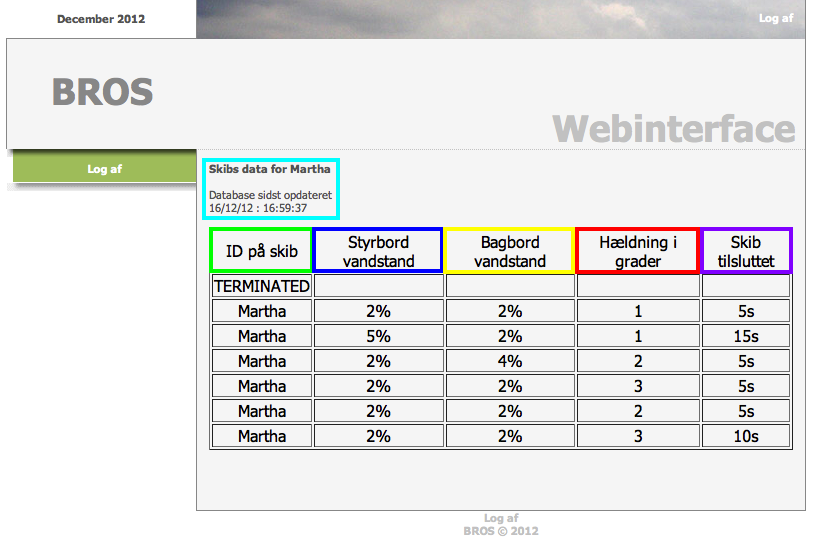
\includegraphics[width=0.8\textwidth]{billeder/web_database}
	\caption{Billed databasen BROS for skibet Martha}
	\label{fig:web_database}
\end{figure}

\begin{table}[H]
\begin{tabular}{p{5cm} p{10cm}}
%\multicolumn{2}{l}{Data fra skib i databasen } \\
\hline
\textcolor{Turquoise}{\textbf{1: Skib er sidst opdateret}}
&Brugeren kan se hvilket skib denne er inde på og hvornår databasen sidst er opdateret.\\ 
\textcolor{green}{\textbf{2: ID på skib}}
&Skibets ID bliver vidst. Hvis at KI lukker tcp forbindelsen vil skibts ID skifte til "TERMINATED".\\
\textcolor{blue}{\textbf{3: Styrbord vandtanksniveau}}
&Der vises hvor meget vand der er i styrbord ballasttank.\\
\textcolor{yellow}{\textbf{4: Bagbord vandtanksniveau}}
&Der vises hvor meget vand der er i bagbord ballasttank.\\
\textcolor{red}{\textbf{5: Hældning i grader}}
&Der vises hvor mange grader sibet hælder i forhold til styrbord.\\
\textcolor{RoyalPurple}{\textbf{6: Skib tilsluttet}}
&Der vise hvor lang tid i secunder der er gået fra overførelsen før til denne.\\
\end{tabular}
\end{table}

\subsection{MySQL}
Som database benyttes MySQL. Denne er en multitreading database som giver mulighed for at flere kan tilgå denne samtid. Det er et færdigt produkt der kan implementeres på de fleste styresystemer. Systemet giver mulighed for at oprette interne databaser med egne taballer til algring af data (se apendix for flere detaljer).
MySQL giver desuden mulighed for at man ved hjælp af php direkte på et website kan oprette databaser og tabeller. Dette betyder at når et nyt skib som ikke har været koblet til systemet før tilkobler serveren. Kan serveren som normalt oprette en fil med dennes data. Når et website med dette implementeret loader filen kan denne se på om dette skib allerede findes, gør det ikke kan den oprette en intern database med tabeller til lagring af data og derefter gemme den nye data. Dette benyttes ikke i denne prototype men systemet er klargjort til det med få ændringer.